\documentclass[fleqn,usenatbib,usedcolumn,useAMS]{mnras}

\usepackage{amsmath,amsfonts}
\usepackage{newtxtext,newtxmath}
\usepackage[T1]{fontenc}
\usepackage{orcidlink}
\usepackage{booktabs}

\DeclareRobustCommand{\VAN}[3]{#2}
\let\VANthebibliography\thebibliography
\def\thebibliography{\DeclareRobustCommand{\VAN}[3]{##3}\VANthebibliography}

\newcommand{\kms}{\,\textrm{km}\,\textrm{s}^{-1}} % kilometres per second
\newcommand{\bibtex}{\textsc{Bib}\!\TeX}

\title[Bayesian characterization of NGC 6383]{Characterizing NGC 6383: A study of pre-main sequence stars, mass segregation, and age using Gaia DR3 and 2MASS}

\author[Pulgar-Escobar et al.]{L.M. Pulgar-Escobar\orcidlink{0009-0008-4359-2444},$^{1}$\thanks{E-mail: \href{mailto:lescobar2019@udec.cl}{lescobar2019@udec.cl}} 
	N.A. Henríquez-Salgado,$^{1}$ Pierluigi Cerulo$^{2}$ and R.E. Mennickent$^{1}$
	\\
	\\
	$^{1}$Departamento de Astronomía, Universidad de Concepción, Casilla 160-C, Concepción, Chile \\
	$^{2}$Departamento de Ingeniería Informática y Ciencias de la Computación, Universidad de Concepción, Chile
}

% These dates will be filled out by the publisher
\date{Accepted XXX. Received YYY; in original form ZZZ}

% Enter the current year, for the copyright statements etc.
\pubyear{2024}

% Don't change these lines
\begin{document}
	\label{firstpage}
	\pagerange{\pageref{firstpage}--\pageref{lastpage}}
	\maketitle
	
	% Abstract of the paper
\begin{abstract}
	This study employs Bayesian analysis and machine learning techniques to analyze the young open cluster NGC 6383 using data from Gaia DR3 and 2MASS. We identified 254 probable cluster members through HDBSCAN and determined the cluster's core and tidal radii. Our results indicate a mean cluster age of $4 \pm 1$ Myr and a distance of $1.107 \pm 0.035$ kpc. The analysis reveals mass segregation, especially among binary stars, and suggests that NGC 6383 is not fully relaxed. We observed a well-defined main sequence and a population of pre-main sequence stars, with a star formation range from $\sim 1$ to $6$ Myr, indicating recent star formation activity.
\end{abstract}

	\begin{keywords}
		open clusters and associations: individual — galaxies: star clusters: general — stars: distances — techniques: photometric — parallaxes — proper motions
	\end{keywords}
	
\section{Introduction}\label{S_intro}
Precise cluster’s members identification is a crucial step when it comes to a correct identification and characterization of the cluster. Various methods have been used for this process  \citep{1930LicOB..14..154T, 1949ApJ...110..117S, 2018AA...610A..30A, 1978MNRAS.182..607F, 1989MNRAS.236..263P, 1991MNRAS.249...76B, 2005AA...438.1163K, 2007AA...462..157P, 1968ArA.....5....1L}, each offering different focuses and sometimes leading to consensus, or discrepancies. Recently, Bayesian analysis implementation on the membership identification, offers a different method to compare or compliment with the ones mentioned.

NGC 6383 \footnote{NGC 6383, also known as NGC 6374 in the New General Catalog \citep{2008hsf2.book..497R} and classified as Collinder 334 and Collinder 335 in the Collinder catalog, was initially misclassified in the original Collinder catalog \citep{1931AnLun...2....1C}.} is a young open cluster situated in the Carina-Sagittarius arm, within the Sh 2-012 star formation region \citep{1959ApJS....4..257S}. It forms part of the larger Sirius OB1 association, along with NGC 6530 and NGC 6531 \citep{2008hsf2.book..497R}. The galactic coordinates of the cluster are $\ell = 355.68^{\circ}$ and $b = 0.05^{\circ}$ \citep{2017A&A...600A.106C}. 

The distance to the cluster has been estimated by various authors, with an upper limit of $2130 ~\mathrm{pc}$ proposed by \cite{1930LicOB..14..154T} and a lower limit of $760~\mathrm{pc}$ and $834~\mathrm{pc}$ suggested by \cite{1949ApJ...110..117S} and \cite{2018AA...610A..30A}, respectively.

 The cluster spans an angular size of $20\,\textrm{arcmin}$ \citep{2013A&A...560A..76M} and is estimated to be between $1.7$ to $5\,\textrm{Myr}$ old \citep{1978MNRAS.182..607F,1989MNRAS.236..263P,1991MNRAS.249...76B,2005AA...438.1163K,2007AA...462..157P}. However, \citet{1968ArA.....5....1L} calculated an age of $20\,\textrm{Myr}$. The reddening $E(B-V) = 0.32 \pm 0.02$ derived by \citet{2008hsf2.book..497R} aligns with previous authors such as \citet{1971AAS....4..241B,1978MNRAS.182..607F,1978MNRAS.184..661L,1985AA...151..391T,1989MNRAS.236..263P,1994RMxAA..29..141F,2007AA...462..157P}, but contradicts \citet{2018AA...610A..30A} who determined a reddening of $E(B-V) = 0.51 \pm 0.03$. This reddening is attributed to a surrounding large shell-structured ionized HII region with a radius of approximately $1\deg$, which was likely ionized by its central star, HD 159176.
 
HD 159176, a double-lined spectroscopic binary composed of O7V type stars located in the projected center of the cluster, is responsible for ionizing the HII region \citep{2016ApJ...832..211P}. The estimated age of HD 159176 is around $2.3-2.8$\,\textrm{Myr} \citep{2010AA...511A..25R}. A careful analysis of both the ages of the cluster and its central star system suggests that the central star predates the cluster itself. Furthermore, \citet{1978MNRAS.182..607F} proposed that HD 159176 initiated star formation in the cluster's core and beyond.

In the study by \citet{2018AA...610A..30A}, it is hypothesized that if the stars numbered as \textit{Star No. 6} are considered to have started to evolve and if HD 159176 is a blue straggler, then the age of the cluster could be between $6$ and $10\,\textrm{Myr}$.

The parameters of the cluster exhibit a wide range of results, contingent on the methodology utilized by the authors in their research. The cluster hosts sources that have recently embarked on the main sequence track, and there are also Pre-Main Sequence Stars (PMS) present \citet{2019MNRAS.484.5102K}. Consequently, the age of the cluster has been a topic of considerable debate.

The implementation of Bayesian analysis and Machine Learning techniques in this study, explores a different method to obtained various parameters for characterizing NGC 6383 and contribute to the debate.

A summary of the historical results can be seen in Table \ref{tab:literature}.

\begin{table*}
	\centering
	\resizebox{\textwidth}{!}{%
		\begin{tabular}{@{}lllllllll@{}}
			\toprule
			\textbf{Reference} &
			\textbf{Members} &
			\textbf{Core Radius} &
			\textbf{Tidal Radius} &
			\textbf{Parallax} &
			\textbf{Distance} &
			\textbf{E(B-V)} &
			\textbf{$(m - M)$} &
			\textbf{Age} \\
			&               & arcmin   & arcmin           & mas               & kpc           & mag           & mag            & Myr          \\ \midrule
			\citet{1930LicOB..14..154T} & $\cdots$      & $\cdots$ & $\cdots$         & $\cdots$          & $2.13$        & $\cdots$      & $\cdots$       & $\cdots$     \\
			\citet{1949ApJ...110..117S} & $\cdots$      & $\cdots$ & $\cdots$         & $\cdots$          & $0.76$        & $\cdots$      & $\cdots$       & $\cdots$     \\
			\citet{1961RGOB...27...61E} & $\cdots$      & $\cdots$ & $\cdots$         & $\cdots$          & $\cdots$      & $0.30$        & $\cdots$       & $\cdots$     \\
			\citet{1967MNRAS.135..377G} & $74$          & $\cdots$ & $\cdots$         & $\cdots$          & $1.38$        & $\cdots$      & $10.68\pm0.54$ & $\cdots$     \\
			\citet{1968PhDT........29E} & At least $21$ & $\cdots$ & $\cdots$         & $\cdots$          & $1.30$        & $0.35$        & $10.6$         & $5$          \\
			\citet{1968ArA.....5....1L} & $\cdots$      & $\cdots$ & $\cdots$         & $\cdots$          & $1.25$        & $\cdots$      & $10.5$         & $\sim 20$    \\
			\citet{1971AAS....4..241B}  & $\cdots$      & $\cdots$ & $\cdots$         & $\cdots$          & $1.07$        & $0.26$        & $10.92$        & $\cdots$     \\
			\citet{1978MNRAS.182..607F} &
			$\cdots$ &
			$1.25$ &
			$\cdots$ &
			$\cdots$ &
			$1.50\pm0.20$ &
			$0.33\pm0.02$ &
			$10.85$ &
			$1.7\pm0.4 $ \\
			\citet{1978MNRAS.184..661L} & $\cdots$      & $\cdots$ & $\cdots$         & $\cdots$          & $1.35$        & $0.35$        & $10.6$         & Up to $5$    \\
			\citet{1985AA...151..391T}  & $\cdots$      & $\cdots$ & $\cdots$         & $\cdots$          & $1.40\pm0.15$ & $0.30\pm0.01$ & $\cdots$       & $\cdots$     \\
			\citet{1989MNRAS.236..263P} & $\cdots$      & $\cdots$ & $\cdots$         & $\cdots$          & $\cdots$      & $0.35$        & $11.65$        & $\sim 4.5$   \\
			\citet{1991MNRAS.249...76B} & $27$          & $\cdots$ & $\cdots$         & $\cdots$          & $1.38$        & $0.34$        & $\cdots$       & $\sim 20$    \\
			\citet{1994RMxAA..29..141F} & $\cdots$      & $\cdots$ & $\cdots$         & $\cdots$          & $1.40$        & $0.33$        & $\cdots$       & $\cdots$     \\
			\citet{2003AA...407..925R}  & $\cdots$      & $\cdots$ & $\cdots$         & $\cdots$          & $\cdots$      & $0.33$        & $10.73$        & $\cdots$     \\
			\citet{2005AA...438.1163K}  & $13$          & $4.80$    & $15$             & $\cdots$          & $0.99$        & $0.3$         & $10.90$        & $5$          \\
			\citet{2007AA...462..157P} &
			$\cdots$ &
			$\cdots$ &
			$\cdots$ &
			$\cdots$ &
			$1.7 \pm 0.3$ &
			$0.29 \pm 0.05$ &
			$\cdots$ &
			Less than $4$ \\
			\citet{2008AA...477..165P}  & $\cdots$      & $\cdots$ & $28.96 \pm 6.63$ & $\cdots$          & $0.99$       & $0.30$        & $10.90$       & $5$          \\
			\citet{2010AA...511A..25R}  & $\cdots$      & $\cdots$ & $\cdots$         & $\cdots$          & $\cdots$      & $\cdots$      & $\cdots$       & $\cdots$     \\
			\citet{2018AA...610A..30A} &
			$\cdots$ &
			$\cdots$ &
			$\cdots$ &
			$\cdots$ &
			$0.83 \pm 0.16$ &
			$0.51 \pm 0.03$ &
			$9.61\pm 0.38$ &
			$\sim 3-10$ \\
			\citet{2019MNRAS.484.5102K} & At least $55$ & $\cdots$ & $\cdots$         & $\cdots$          & $\cdots$      & $\cdots$      & $\cdots$       & $2.8\pm 1.6$ \\
			\citet{2021ApJ...923..129J} & $284$         & $\cdots$ & $\cdots$         & $0.93 \pm 0.09$ & $1.07$       & $\cdots$      & $\cdots$       & $\cdots$     \\
			\citet{2022ApJS..262....7H} & $\cdots$      & $\cdots$ & $\cdots$         & $0.88 \pm 0.05$ & $\cdots$      & $0.45$        & $\cdots$       & $3.5$        \\
			\citet{2024arXiv240305143H} & $322$         & $2.49$  & $22.73$         & $0.89 \pm 0.08$ & $1.1$         & $0.38$        & $10.18$       & $\sim 4$     \\
			\citet{2024arXiv240301030P} &
			$266$ &
			$1.21 \pm 0.13$ &
			$29.72 \pm 7.69 $ &
			$0.92 \pm 0.06$ &
			$1.10 \pm 0..04$ &
			$0.47 \pm 0.03$ &
			$10.90 \pm 0.33$ &
			$\sim 1-4$ \\ \bottomrule
		\end{tabular}%
	}
	\caption{Comprehensive historical review of observed parameters for the open cluster NGC 6383, gathered from various studies. The table details the number of cluster members, core and tidal radii (in arcminutes), parallax (in milliarcseconds), distance (in kiloparsecs), E(B-V) color excess, distance modulus $(m - M)$ (in magnitudes), and estimated ages (in millions of years). This summary provides a comparative analysis of how measurements and interpretations of NGC 6383 have evolved over time.}
	\label{tab:literature}
\end{table*}
\begin{figure}
	\centering
	
\includegraphics[width=\columnwidth]{Figures/probabilies_post_sigmaclip.pdf}
	\caption{Membership probability of potential NGC 6383 members is plotted against their $G$ magnitudes, with colors representing astrometric fidelity. Each data point indicates a star, using a color gradient from blue to red to reflect the varying reliability of astrometric measurements. The horizontal dashed line at a probability of $0.6$ marks the threshold for probable cluster membership. As shown in the figure, stars with fainter magnitudes tend to have lower astrometric fidelity, which becomes more evident for stars with magnitudes fainter than 18.}
	\label{fig:probabilities}
\end{figure}
\section{Methodology}
We acquired data from the \textit{Gaia} third Data Release (DR3) \citep{2016A&A...595A...1G,2022arXiv220800211G}, executing a cone search of $40~\mathrm{arcmin}$ radius on the \textit{Gaia} archive, yielding $23740$ sources. We restricted the initial selection filtered sources to parallax ranges between $0.75$ and $1.1~\mathrm{mas}$—based on limits established in \citet{2024arXiv240301030P}.

\begin{figure}
	\centering
	
\includegraphics[width=\columnwidth]{Figures/center_determination_paper.pdf}
	\caption{Spatial distribution of potential members with a probability of at least 60 percent of NGC 6383 in Right Ascension $(\alpha)$ and Declination $(\delta)$, plotted against membership probability. Each point's color indicates the probability of cluster membership, ranging from blue (lower probability) to red (higher probability). Concentric contour lines represent levels of Kernel Density Estimation (KDE) with an exponential kernel, revealing the density gradient of the points. The central coordinates of the cluster are marked by white dashed lines at $ \alpha = 263.6826^\circ $ and $ \delta = -32.5838^\circ $, which correspond to the density peak within the plotted area. A scale bar of 5 parsecs is included at the bottom right to provide a reference for spatial scale.}
	\label{fig:center}
\end{figure}
To enhance data reliability, we applied astrometric fidelity parameters from \cite{2022MNRAS.510.2597R}. This parameter, derived from a neural network analysis of $17$ \textit{Gaia} catalog metrics, assesses the astrometric solution's trustworthiness. Sources with an astrometric fidelity above $0.5$ were retained, narrowing the selection to $15480$ sources, which is the $65$ per cent of the initial data set.

Subsequent refinement ensured inclusion of only sources with the position $(\alpha,\delta,\ell,b)$, proper motions $(\mu_{\alpha*},\mu_\delta)$, parallax ($\varpi$) and the magnitudes $(G, G_\mathrm{BP}, G_\mathrm{RP})$, finalizing the dataset at $15276$ sources. Systematic parallax offsets identified in \citet{2021A&A...649A...2L} were corrected using the \href{https://pypi.org/project/gaiadr3-zeropoint/}{\textsc{Gaiadr3\_zeropoint}} package. Moreover, to address the bias in proper motion for bright sources ($\mathrm{G}<13~\mathrm{mag}$), as discussed by \citet{2021A&A...649A.124C}, we applied a magnitude-based correction for sources with $\mathrm{G} = 11-13~\mathrm{mag}$, compensating for up to $80~\mathrm{\mu as\,yr^{-1}}$ discrepancy between the frames of reference for bright and faint sources.

Furthermore, for the infrared part of the spectrum,  we obtained the $J$, $H$, and $K_s$ magnitudes from \textsc{Two Micron All-Sky Survey} (2MASS) \citep{2006AJ....131.1163S}. A cross-match was performed to obtain a final list of sources, using the pre-computed crossmatch from Gaia DR3, as explained in \citet{2022gdr3.reptE..15M}. The table used for the crossmatch was \texttt{tmass\_psc\_xsc\_best\_neighbour}, giving $5351$ crossmatched sources with a separation distance of less or equal than $0.3~\textrm{arcsec}$ . The join type was only adding the avalaible 2MASS data to the Gaia data, keeping the original $15480$ sources.

\subsection{\sc COSMIC}
Characterization Of Star clusters using Machine learning Inference and Clustering (\textsc{COSMIC}) developed by Lucas Pulgar-Escobar et al. (in prep.), is a suite of functions designed for analyzing open clusters. Utilizing unsupervised machine learning algorithms, \textsc{COSMIC} processes extensive datasets, such as those from \textit{Gaia}, to identify fundamental parameters of open clusters through clustering techniques and Bayesian estimation. As an open-source program, it is developed in \textsc{Python} 3.12 and integrates \textsc{PyMC} 5\footnote{\href{www.pymc.io}{www.pymc.io}}, a \textsc{Python} library specialized in Bayesian analysis.

The PyMC library aims to modernize and simplify Bayesian modeling. It offers a user-friendly interface for setting the prior distribution, generally a Normal distribution, and executes the sampling process efficiently. One of the key advantages of using PyMC is its implementation of the No-U-Turn Sampler (NUTS), an advanced MCMC algorithm that allows for efficient exploration of high-dimensional parameter spaces.

The NUTS algorithm builds upon Hamiltonian Monte Carlo (HMC) techniques, simulating a physical system to generate proposals. These proposals are based on the topology of the posterior distribution, allowing for an adaptive and balanced exploration of the parameter space. The algorithm terminates when a U-turn is detected, which serves as an indicator that the space has been sufficiently explored. A U-turn is detected when the trajectory of the sample path starts to double back on itself, indicating that it is moving in the opposite direction.

This efficiency and adaptability give NUTS an edge over traditional methods like Metropolis-Hastings and Gibbs sampling, which are often constrained by the shape of the distribution or the dimensions being considered \citep{phan2019composable}.
 
\begin{figure}
	\centering
	
\includegraphics[width=\columnwidth]{Figures/proper_motion_2d_paper.pdf}
	\caption{Proper motions of sources with a probability of at least 60 percent of NGC 6383 in Right Ascension ($\mu_{\alpha}^*$) and Declination ($\mu_{\delta}$), color-coded by membership probability. The diagram uses hues transitioning from blue (lower probabilities) to red (higher probabilities), overlaid with density contours of proper motions. The contours illustrate the density gradient of proper motions. The center of proper motion distribution is marked by a blue cross, indicating the inferred mean proper motion values $(\mu_{\alpha}^*, \mu_{\delta}) = (2.5418, -1.7126)~\mathrm{mas}\,\mathrm{yr}^{-1}$, with corresponding orange dashed lines highlighting these central coordinates.}
	\label{fig:proper_motion}
\end{figure}
\subsubsection{Membership determination}
To identify potential members of NGC 6383, we employed the Hierarchical Density-Based Spatial Clustering of Applications with Noise (\textsc{HDBSCAN}) algorithm \citep{10.1007/978-3-642-37456-2_14}, known for its effectiveness in identifying clusters of varying densities and sizes without requiring a predetermined number of clusters \citep{2021A&A...646A.104H}. This density-based clustering method, which constructs a hierarchical representation of the data \citep{McInnes2017}, is particularly adept at handling different cluster shapes and sizes while distinguishing noise points. Its capacity to automatically determine the optimal cluster count makes \textsc{HDBSCAN} an ideal choice for this analysis, offering significant benefits over traditional clustering algorithms, especially in terms of robustness against noisy data and outliers.
\begin{figure*}
	\centering
	
\includegraphics[width=\textwidth]{Figures/parallax_determination_paper.pdf}
	\caption{\emph{Left panel:} Histograms display parallax measurements for NGC 6383. \textit{Used Parallax} in red represents measurements with fractional parallax errors less than 0.1, \textit{Parallax} in orange includes all data, and \textit{Non-Used Parallax} in green for sources with a fractional parallax error greater than 0.1. The blue curve shows a Gaussian fit to the used parallax data, with the mean parallax value $ \mu_{\varpi} = 0.908 \pm 0.004 \, \mathrm{mas} $ marked by the dashed green line. \emph{Middle panel:} G magnitude versus parallax values, with data utilized for distance estimation in blue and discarded due to having a fractional parallax error greater than 0.1 in red. Grey error bars illustrate the uncertainty in parallax measurements, especially pronounced at fainter magnitudes. \emph{Right panel:} Histograms of distances derived from the inverse of parallax to differentiate between used (red) and all measured (orange) parallaxes, including non-used (green). The central dashed blue line marks the mean sampled distance ($ \mu_{d} = 1.107 \pm 0.035 \, \mathrm{kpc} $), with its standard deviation area shaded in blue.}
	\label{fig:parallax_distance}
\end{figure*}
After narrowing the data to a final subset of $15480$ sources, \textsc{HDBSCAN} was applied, focusing on proper motions as the primary clustering parameters.

To refine our selection of hyperparameters for optimal cluster identification, we utilized a systematic approach. This involved iterative testing of various minimum cluster sizes to find the setup that enhances cluster size while ensuring high cluster separation strength, as indicated by the maximum $\lambda$ value. Our strategy aimed at selecting leaf clusters to generate numerous small, homogeneous groups, aiming to include the maximum number of stars without compromising the separation strength. While this approach risks increasing false positives, it is essential for capturing all potential cluster members, particularly for studying tidal sources. To mitigate this risk, we derived a pseudo-probability metric. This metric was calculated by determining the frequency with which a source was identified as a cluster member across multiple iterations, divided by the total number of iterations, and then multiplying this value by the HDBSCAN membership probability. Sources with a resulting probability greater than 0.5 were retained. The variation in cluster sizes and the threshold for minimum cluster size are depicted in Fig. \ref{fig:min_cluster_size}. Additionally, we used a Euclidean metric for clustering based on proper motions, finding that while the Haversine metric was tested, it produced non-physical clusters.

Finally, we used the \textsc{AstroPy Sigma Clipping} \citep{astropy:2013,astropy:2018,astropy:2022} utility to perform a $2\sigma$ clipping method around the mode in order to obtain the final likely members of the cluster.

\subsubsection{Parallax and Distance Estimation}
Distance estimation from parallax is challenging due to measurement errors, and transforming parallax to distance is not straightforward and involves significant uncertainties, deviating from the simple \textit{inverse of the parallax} approach \citep{2015PASP..127..994B,2021AJ....161..147B}. A crucial aspect is choosing an appropriate prior distribution. When analyzing the parallax measurements of stars within an open cluster and assuming a simplified one-dimensional perspective, observing the distribution of parallax sources, we can assume that it follows a normal distribution. For accuracy, our analysis only includes members with fractional parallax errors under $0.1$.

Our hierarchical model begins by calculating an initial average distance $(\mu_{\mathrm{prior}})$ from the observed parallaxes. The cluster's mean distance follows $\mathcal{U}(0.5\mu_{\mathrm{prior}},1.5\mu_{\mathrm{prior}})$ as a prior, with an assumed normal likelihood.

\begin{figure}
	\centering
	
\includegraphics[width=\columnwidth]{Figures/king_profile_logscale.pdf}
	\caption{Radial density profile of NGC 6383 shown in logarithmic scale. The plot overlays the observed stellar density (blue points) against the King model (solid fuchsia line). Dashed red and dotted red lines mark the core radius ($ R_c = 1.944 \, \text{arcmin} $) and the tidal radius ($ R_t = 40.713 \, \text{arcmin} $), respectively. The dash-dot green line represents the $ b $ parameter of the background level. The shaded area in blue indicates the $ 1\sigma $ uncertainty range of the King profile.}
	\label{fig:king}
\end{figure}
\subsubsection{Proper motions}
To estimate the distribution of cluster members' proper motions, we model them using a two-dimensional normal distribution. 

A normal prior distribution was assigned to the mean proper motions $\left[\overline{\mu_\alpha},\overline{\mu_\delta}\right]$, based on frequentist means and standard deviations. The standard deviations are modeled using a HalfNormal distribution, while the correlation coefficient between the proper motions is uniformly distributed over the interval $[-1, 1]$. 

We also estimated the mean projected velocity of the cluster, defined as the square root of the sum of squares of the proper motion components.
\begin{figure*}
	\centering
	
\includegraphics[width=\textwidth]{Figures/real_sky.pdf}
	\caption{Spatial distribution of NGC 6383 sources overlaid on a DSS2-red image, centered on the calculated cluster center marked by a blue cross. The image details various structural and dynamical boundaries of the cluster as follows: the tidal radius $ R_t $ is depicted with a dashed dark slate grey line, the core radius $ R_c $ with a solid dark blue line, the half-light radius $ R_{\mathrm{hl}} $ with a dash-dot magenta line, the half-mass radius $ R_{\mathrm{hm}} $ with a solid yellow line, the Hill radius $ R_{\mathrm{hill}} $ with a dashed orange line, and the gravitational bound radius $ R_{\mathrm{bound}}$ with a solid red line. A scale bar indicating 5 parsecs is positioned at the bottom right to provide spatial reference relative to the cluster scale.}
	\label{fig:real_sky}
\end{figure*}
\subsubsection{Center determination}
To  determine the cluster's center, we used a weighted Kernel Density Estimation (KDE) from \textsc{sci-kit learn} \citep{scikit-learn}, assigning weights inversely proportional to the distance from the mean proper motion. Optimal KDE parameters were determined through Grid Search Cross-Validation within the package, exploring a range of bandwidths—from the mean positional error to the search cone radius—and all kernel types. The location of maximum density was designated as the cluster's center.
\subsubsection{Radial density profile}
To determine structural parameters of the cluster, we utilized the \citet{1962AJ.....67..471K} density profile.

The numerical density $\rho$, was computed by dividing the cluster area into concentric annuli, each containing an equal number of stars. The number of annuli, $K$, adheres to the equiprobable bin rule ($K = 2n^{2/5}$), where $n$ is the star count within the cluster. Fitting King's model to the density data allows for estimating the structural parameters' posterior distributions.

Priors for the model parameters were set as follows: $b \sim \mathcal{U}(0, 2\rho_{\mathrm{min}})$, $k \sim \mathcal{U}(0, 2\rho_{\mathrm{max}})$, $R_c \sim \mathcal{U}(0, 0.8R_t)$, and $R_t \sim \mathcal{U}(R_c, 1.5T_{\mathrm{max}})$, where $T_{\mathrm{max}}$ represents the highest value among Hill radius and gravitational bound radius. This ensures the chosen parameter space for $R_c$ and $R_t$ is within astrophysical valid limits. 

The Hill Radius $(R_\mathrm{hill})$  can be calculated following the methodology outlined by \citet{2019A&A...627A.119C}:
\begin{equation}
R_\mathrm{hill} = R_{\mathrm{gc}} \times \left(\frac{m_c}{3M_{\mathrm{gc}}}\right)^{1/3}
\end{equation}
where $ R_{\mathrm{gc}} $ denotes the galactocentric distance, $ m_c $ the cluster mass from \citet{2024arXiv240305143H}, with a value of $902.27~\mathrm{M_{\odot}}$, and $ M_{\mathrm{gc}} $ the Galactic mass within the cluster's orbit calculated as
\begin{equation}
	M_{\mathrm{gc}} = 2  \times 10^8\,M_\odot \left(\frac{R_G}{30\,\mathrm{pc}}\right)^{1.2}.
\end{equation}
Moreover, the gravitationally bound radius was estimated using the method described by \citet{1998MNRAS.299..955P}, which considers the cluster mass and Oort constants, using the formula
\begin{equation}
	r_\mathrm{bound} = \left( \frac{GM_{\mathrm{total}}}{2(A-B)^2} \right)^{1/3},
\end{equation}
where $G$ is the gravitational constant, and $A$ and $B$ are the Oort constants, with values from \citet{2017MNRAS.468L..63B}.
\begin{table}
	\centering
	\resizebox{\columnwidth}{!}{%
		\begin{tabular}{llc}
			\hline
			\textbf{Parameter}                      & \textbf{Value}      & \textbf{Unit}                      \\ \hline
			Distance $(\varpi)$                     & $1.107 \pm 0.035$   & $\mathrm{kpc}$                     \\
			Distance (D.M.)                         & $1.211_{0.858}^{1.709}$   & $\mathrm{kpc}$                     \\
			Distance Modulus                        & $10.416 \pm 0.748$    & $\mathrm{mag}$                     \\
			Age                                     & $4 \pm 1$           & $\mathrm{Myr}$                     \\
			Stellar formation range                 & $1 - 6$             & $\mathrm{Myr}$                     \\
			Metallicity ($Z$)                       & $0.023 \pm 0.008$   & -                                  \\
			Parallax $(\varpi)$                     & $0.908 \pm 0.004$   & $\mathrm{mas}$                     \\
			Number of members                       & $254$               & $\mathrm{stars}$                   \\
			Absorption $(A_V)$                      & $1.221 \pm 0.241$   & $\mathrm{mag}$                     \\
			Galactocentric distance $R_\mathrm{GC}$ & $7.197$             & $\mathrm{kpc}$                     \\
			Core Radius $(R_c)$                     & $1.943 \pm 0.1857$  & $\mathrm{arcmin}$                  \\
			Background $(b)$                        & $0.011 \pm 0.0062$  & $\mathrm{stars\,arcmin^{-2}}$      \\
			Tidal Radius $(R_t)$                    & $40.712 \pm 14.379$ & $\mathrm{arcmin}$                  \\
			Center Density $(k)$                    & $4.902 \pm 0.413$   & $\mathrm{stars\,arcmin^{-2}}$      \\
			Hill radius                             & $28.608$            & $\mathrm{arcmin}$                  \\
			Gravitational bound radius              & $42.842$            & $\mathrm{arcmin}$                  \\
			Cluster Center R.A.                     & $263.683 \pm 0.112$ & $\mathrm{deg}$                     \\
			Cluster Center DEC.                     & $-32.584 \pm 0.112$ & $\mathrm{deg}$                     \\
			Proper Motion R.A.                      & $2.542 \pm 0.0094$  & $\mathrm{mas\,yr^{-1}}$            \\
			Proper Motion DEC.                      & $-1.713 \pm 0.0086$ & $\mathrm{mas\,yr^{-1}}$            \\
			Half-Mass Relaxation time               & $9.808$             & $\mathrm{Myr}$                     \\
			Radial Velocity                         & $-0.67 \pm 33.056$  & $\mathrm{km\,s^{-1}}$              \\
			Concentration Parameter $(C)$           & $3.042$             & -                                  \\
			Young Stellar Objects (YSOs)            & $53$                & $\mathrm{stars}$                   \\
			$Y_{\text{frac}}$                       & $0.18$              & -                                  \\
			Minimum Segregation Time                & $1.364$             & $\mathrm{Myr}$                     \\ \hline
		\end{tabular}%
	}
	\caption{Summary of derived parameters for NGC 6383, focusing on members with at least a 60 percent membership probability. Key measurements include distances assessed through parallax and distance modulus, mean age and stellar formation range, metallicity, and total stellar membership. The table also outlines structural attributes such as core and tidal radii, absorption, and galactocentric distance, complemented by dynamic properties like proper motions, radial velocities, concentration parameters, specific radius measurements, the number of identified Young Stellar Objects (YSOs), the fraction of YSOs, and the minimum segregation time.}
	\label{tab:ngc6383_results}
\end{table}
\begin{figure}
	\centering
	
\includegraphics[width=\columnwidth]{Figures/ngc6383_cmd.pdf}
	\caption{CMD of NGC 6383, depicting the classification of cluster members and their evolutionary states, determined using the Sagitta. The mean fit isochrone is denoted by the dashed black curve, while the median fit is shown with a dotted black line. Red stars indicate PMS Members with membership probabilities and PMS probabilities $\geq 0.6$. Orange diamonds represent PMS Probable Members with probabilities and PMS probabilities $\leq 0.6$. Blue stars signify MS Members with membership probabilities $\leq 0.6$ and PMS probabilities $< 0.6$, and blue-violet diamonds are for MS Probable Members with probabilities $> 0.6$ and PMS probabilities $< 0.6$. The shaded area around the isochrone visualizes the uncertainty within the parameter fits, represented by a normal distribution. Additionally, error bars, plotted at regular intervals along the color axis, mean color error.}
	\label{fig:cmd}
\end{figure}
\subsection{AsTeCA}
AsTeCA, or Automated Stellar Cluster Analysis \citep{2015A&A...576A...6P}, is an open-source Python tool designed to automate standard tests for determining basic parameters of stellar clusters. For accurate estimation of a cluster's metallicity, age, and extinction values, we employed AsTeCA's isochrone fitting process. We utilized the \textsc{MIST} isochrones \citep{2016ApJS..222....8D, 2016ApJ...823..102C} along with the photometric systems of \textsc{Gaia} EDR3 and \textsc{2MASS}. The Initial Mass Function (IMF) settings followed \citet{2014ApJ...796...75C}, with fixed values for $\alpha = 0.09$, $\beta = 0.94$, and differential reddening set to zero. 

The priors for metallicity $Z$, logarithmic age, and absorption $A_V$ were defined as uniform distributions ranging from $[0.01, 0.045]$, $[5, 10.3]$, and $[0.5,2]$, respectively, aligned with findings from \cite{2024arXiv240301030P}. The distance modulus was modeled as $\mathcal{N}(10.3, 0.2)$, with the mean value following the expected distance modulus obtained from the parallax. We opted for the median solution and chose to utilize the No-U-Turn Sampler (NUTS) from PyMC, prioritizing its efficiency over the Approximate Bayesian Computation (ABC) suggested by ASteCA.
\begin{figure*}
	\centering
	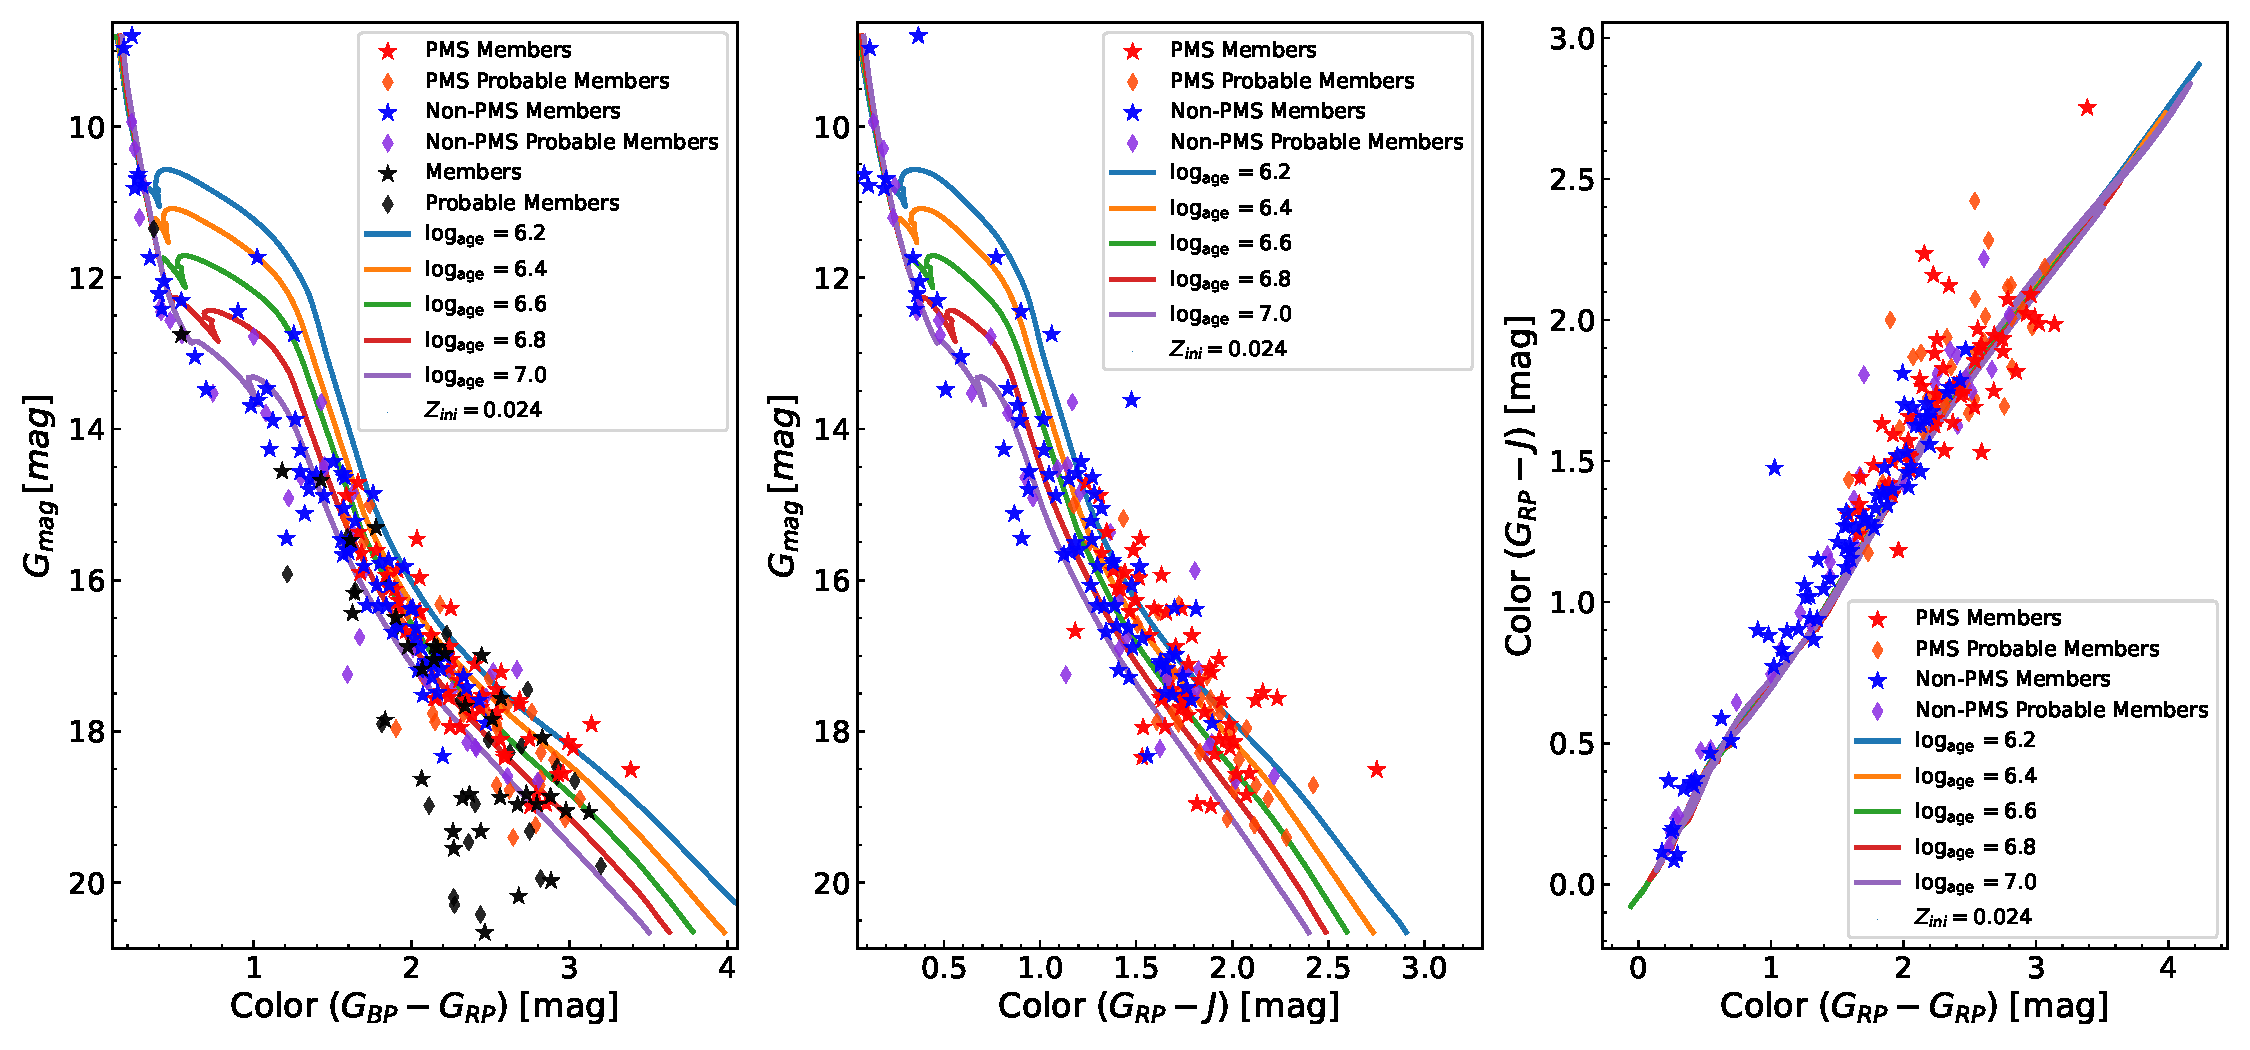
\includegraphics[width=\textwidth]{Figures/ngc6383_cmd_various.pdf}
	\caption{\emph{Left panel:} Color-Magnitude Diagram (CMD) for NGC 6383 showing $G_{\text{mag}}$ against $G_{\text{BP}} - G_{\text{RP}}$ with isochrones for $\log(\text{age})$ ranging from 6.2 to 7.0. \emph{Middle panel:} CMD using $G_{\text{mag}}$ versus $G_{\text{RP}} - J$. \emph{Right panel:} Color-Color diagram $G_{\text{RP}} - G_{\text{RP}}$ against $G_{\text{RP}} - J$ with the equivalent color-color isochrones. Red stars represent PMS Members, orange diamonds indicate PMS Probable Members, blue stars are MS Members, and blue-violet diamonds show MS Probable Members, as in Fig. \ref{fig:cmd}. Isochrones are color-coded to represent different ages, highlighting the evolutionary progression of members within NGC 6383. Each plot includes a legend indicating the initial metallicity ($Z_{\text{ini}} = 0.023$).
	}
	\label{fig:cmd_ngc6383_various}
\end{figure*}
\subsection{Sagitta}
Sagitta is a neural network designed to classify stars as pre-main sequence (PMS) and estimate their ages, trained with data from Gaia DR2 and the 2MASS. It incorporates three convolutional neural networks each dedicated to determining stellar extinction ($A_v$), PMS probability, and estimating stellar ages. Sagitta's age estimation is applicable for young stars up to $\sim 80~\mathrm{Myr}$ and relies on inputs including Gaia parallaxes, and average line-of-sight extinction \citep{2021AJ....162..282M}.

This tool's efficacy stems from its training on a well-curated dataset of PMS stars within moving groups \citep{2020AJ....160..279K}, and is supplemented by various literature sources that have provided previously measured ages. Sagitta uniquely offers stability in age predictions across G, K, and M-type stars within the same population, surpassing traditional isochrone techniques in consistency \citep{2023AJ....165..182K}.

By identifying PMS stars and their ages within NGC 6383, it allows for a nuanced understanding of the cluster's star-forming history. It is important to note that Sagitta is most reliable for PMS stars; the photometry of higher-mass stars that have reached the main sequence is not indicative of their age, limiting the model's applicability to stars that remain in the PMS stage.
\begin{figure}
	\centering
	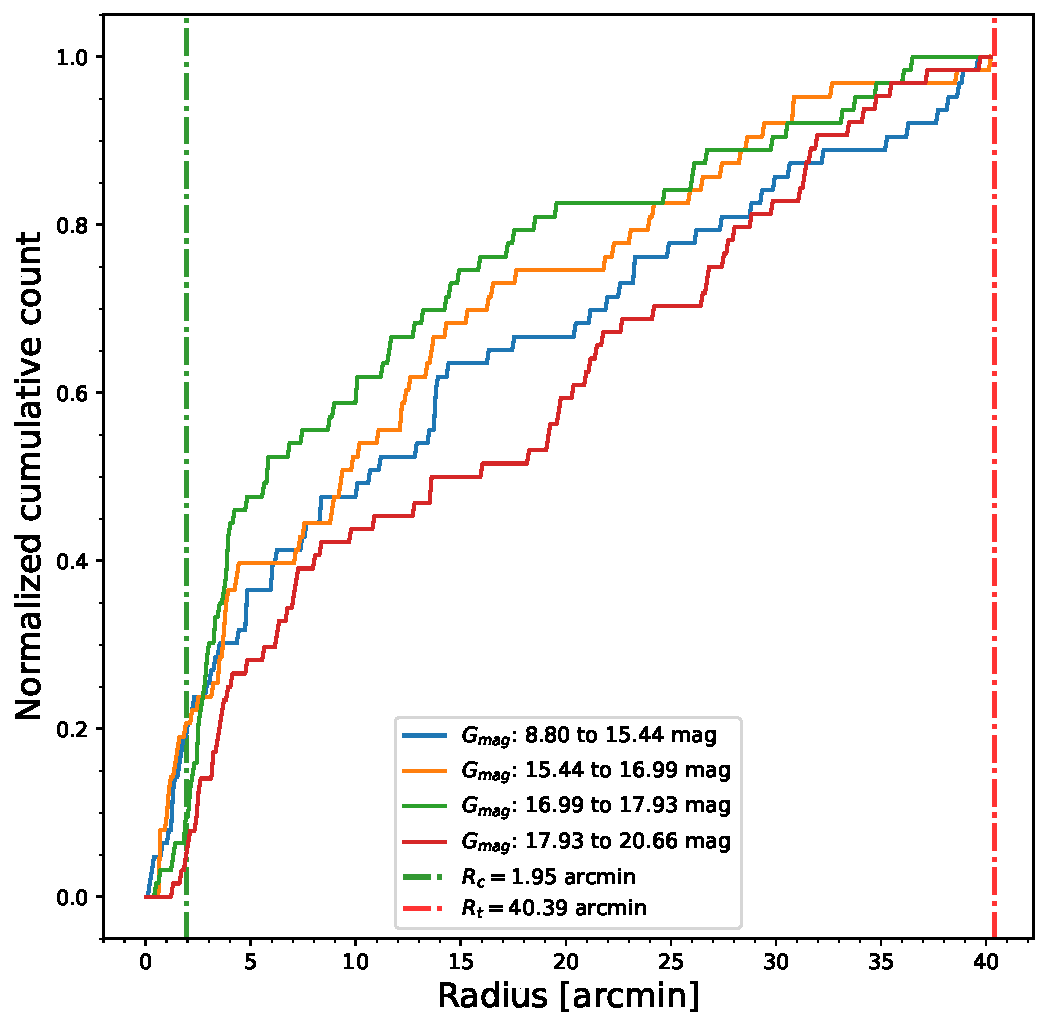
\includegraphics[width=\columnwidth]{Figures/cumulative_by_brightness_paper.pdf}
	\caption{Normalized cumulative counts of stars within NGC 6383 are plotted against radial distance from the cluster center for different brightness ranges, segmented into quartiles of $G_{\text{mag}}$ from the brightest at 8.80 mag to the faintest at 20.66 mag. The green dashed line at $R_c = 1.94$ arcmin marks the core radius, and the red dashed line at $R_t = 40.71$ arcmin denotes the tidal radius, illustrating the spatial distribution of stars with varying brightness within these boundaries. See the text for more reference.}
	\label{fig:cumulative_luminosity}
\end{figure}
\section{Results}
In this section, we report the primary findings of our study, focusing on the mode of the distributions for members with a membership probability of at least $60$ per cent.

Table \ref{tab:ngc6383_results} summarizes the derived parameters for sources with membership probabilities exceeding $60$ per cent. The probability distribution for these sources is illustrated in Fig. \ref{fig:probabilities}. The condensed cluster tree is depicted in Fig. \ref{fig:condensed_cluster_tree}, and Fig. \ref{fig:center} indicates the cluster's center. The proper motions of the cluster members are shown in Fig. \ref{fig:proper_motion}, while Fig. \ref{fig:parallax_distance} shows the distance and parallax estimations. The structural parameters of the cluster, alongside the fitted King Profile, are presented in Fig. \ref{fig:king}. Fig. \ref{fig:real_sky} provides a visualization of the tidal radius, core radius, half-light radius, half-mass radius, the Hill radius, and the gravitational bound radius. Finally, Fig. \ref{fig:cmd} displays the best-fit isochrone and the Color-Magnitude Diagram (CMD) of NGC 6383.

Applying the HDBSCAN algorithm returned several clusters, predominantly composed of non-physical clusters. However, one significant cluster is recognized, distinguished by its proper motions. This cluster contained $701$ sources initially, and after applying a $2\sigma$ clipping based on the methodology outlined, $321$ sources were retained.
\begin{figure}
	\centering
	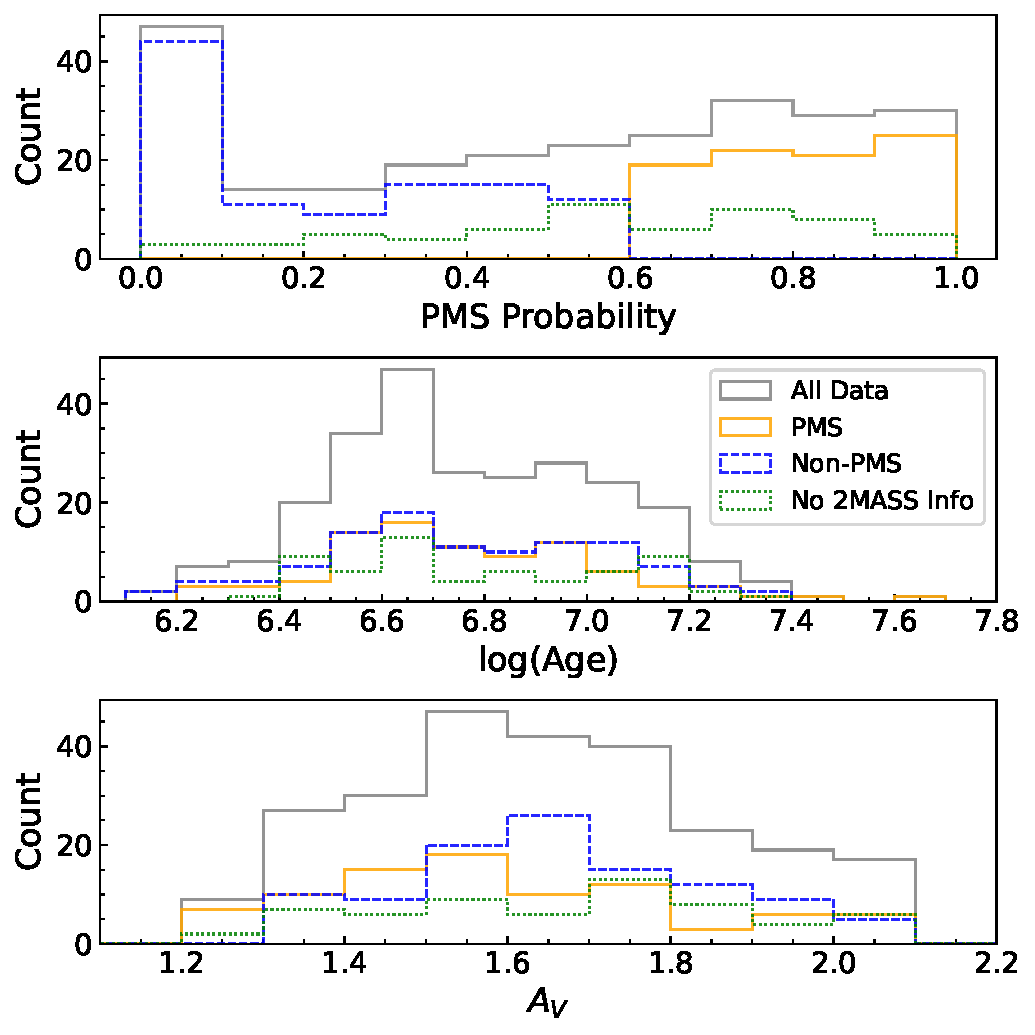
\includegraphics[width=\columnwidth]{Figures/pms_stats.pdf}
	\caption{Histograms of parameters obtained with Sagitta for NGC 6383 potential members with a PMS probability over 60 percent. \emph{Upper panel:} Distribution of PMS probability values, indicating the likelihood of stars being pre-main-sequence stars. \emph{Middle panel:} Distribution of logarithmic age values, illustrating the range and frequency of star ages within the cluster. \emph{Lower panel:} Distribution of visual extinction values ($A_V$), representing the amount of dust extinction affecting the observed stars.}
	\label{fig:pms_sagitta_stats}
\end{figure}
Regarding membership probabilities, NGC 6383 has $321$, $254$, $202$, and $161$ members with probabilities above $50$, $60$, $70$, and $80$ per cent respectively. Correspondingly, $288$, $236$, $191$, and $153$ of these members are brighter than $G=19\,\mathrm{mag}$.

The central position of the cluster in equatorial coordinates is $263.6826 \pm 0.1122\,^\circ$ in RA and $-32.5838 \pm 0.1122\,^\circ$ in DEC. These errors are calculated from the quadratic sum of the mean errors in RA and DEC and the optimal KDE bandwidth. The mean proper motion values are $2.5419 \pm 0.0094\,\mathrm{mas\,yr^{-1}}$ in RA and $-1.7127 \pm 0.0086\,\mathrm{mas\,yr^{-1}}$ in DEC, with dispersions of $0.1532$ and $0.1383$ respectively, which align with the acceptable values from \citet{2023MNRAS.526.4107P}. The projected velocity is calculated as $3.068 \pm 0.009\,\mathrm{mas\,yr^{-1}}$.

The mean parallax derived is $0.908 \pm 0.004\,\mathrm{mas}$, with a mean sampled distance of $1.107 \pm 0.035\,\mathrm{kpc}$. These values slightly deviate from the results obtained by earlier studies \citep{1930LicOB..14..154T,1949ApJ...110..117S,1978MNRAS.182..607F,1985AA...151..391T,2007AA...462..157P} but are consistent with more recent findings \citep{1971AAS....4..241B,2005AA...438.1163K,2008AA...477..165P,2021ApJ...923..129J,2022ApJS..262....7H,2024arXiv240301030P,2024arXiv240305143H}.

Radial velocities are estimated with a median of $-0.67 \pm 33.056\,\mathrm{km}\,\mathrm{s}^{-1}$ using $16$ clustered sources with probabilities above $60$ per cent and a binary probability lower than $60$ per cent. The substantial standard deviation primarily stems from the limited availability of radial velocity data—only $6.299$ per cent of our Gaia-selected sources. Figure \ref{fig:radial_velocities} illustrates the sources with available radial velocities, their magnitudes, and the amplitude of their radial velocities.
\begin{figure}
	\centering
	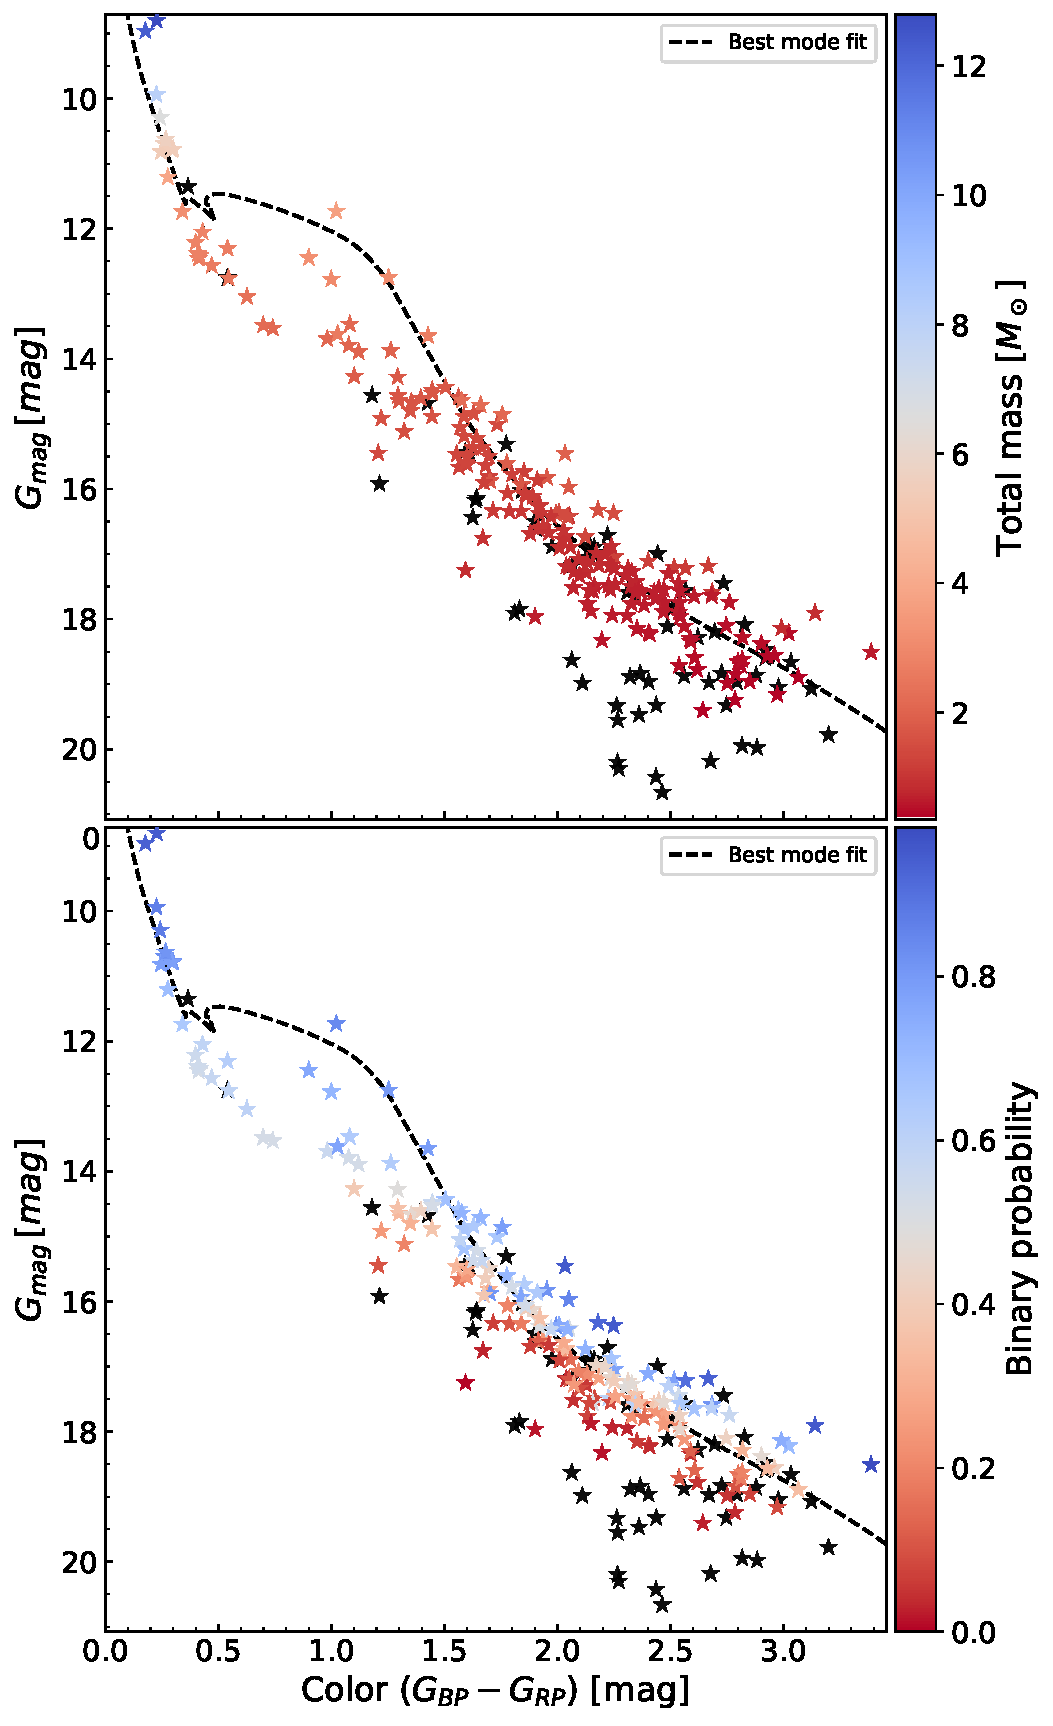
\includegraphics[width=\columnwidth]{Figures/ngc6383_mass_binary.pdf}
	\caption{\emph{Upper Panel:} Color-magnitude diagram displaying probable members and members of NGC 6383, color-coded by total mass, which ranges from lower to higher mass (red to blue). The dashed black line represents the best mean fit isochrone, and the dotted black line represents the best median fit isochrone, illustrating the evolutionary track inferred for the cluster. The total mass is calculated as the sum of the two components if the binary probability is greater than 0.7. \emph{Lower Panel:} Same stars as in the upper panel, now color-coded by binary probability, illustrating the likelihood of binary systems within these stars from low to high (red to blue).}
	\label{fig:cmd_mass_binary}
\end{figure}
\begin{figure*}
	\centering
	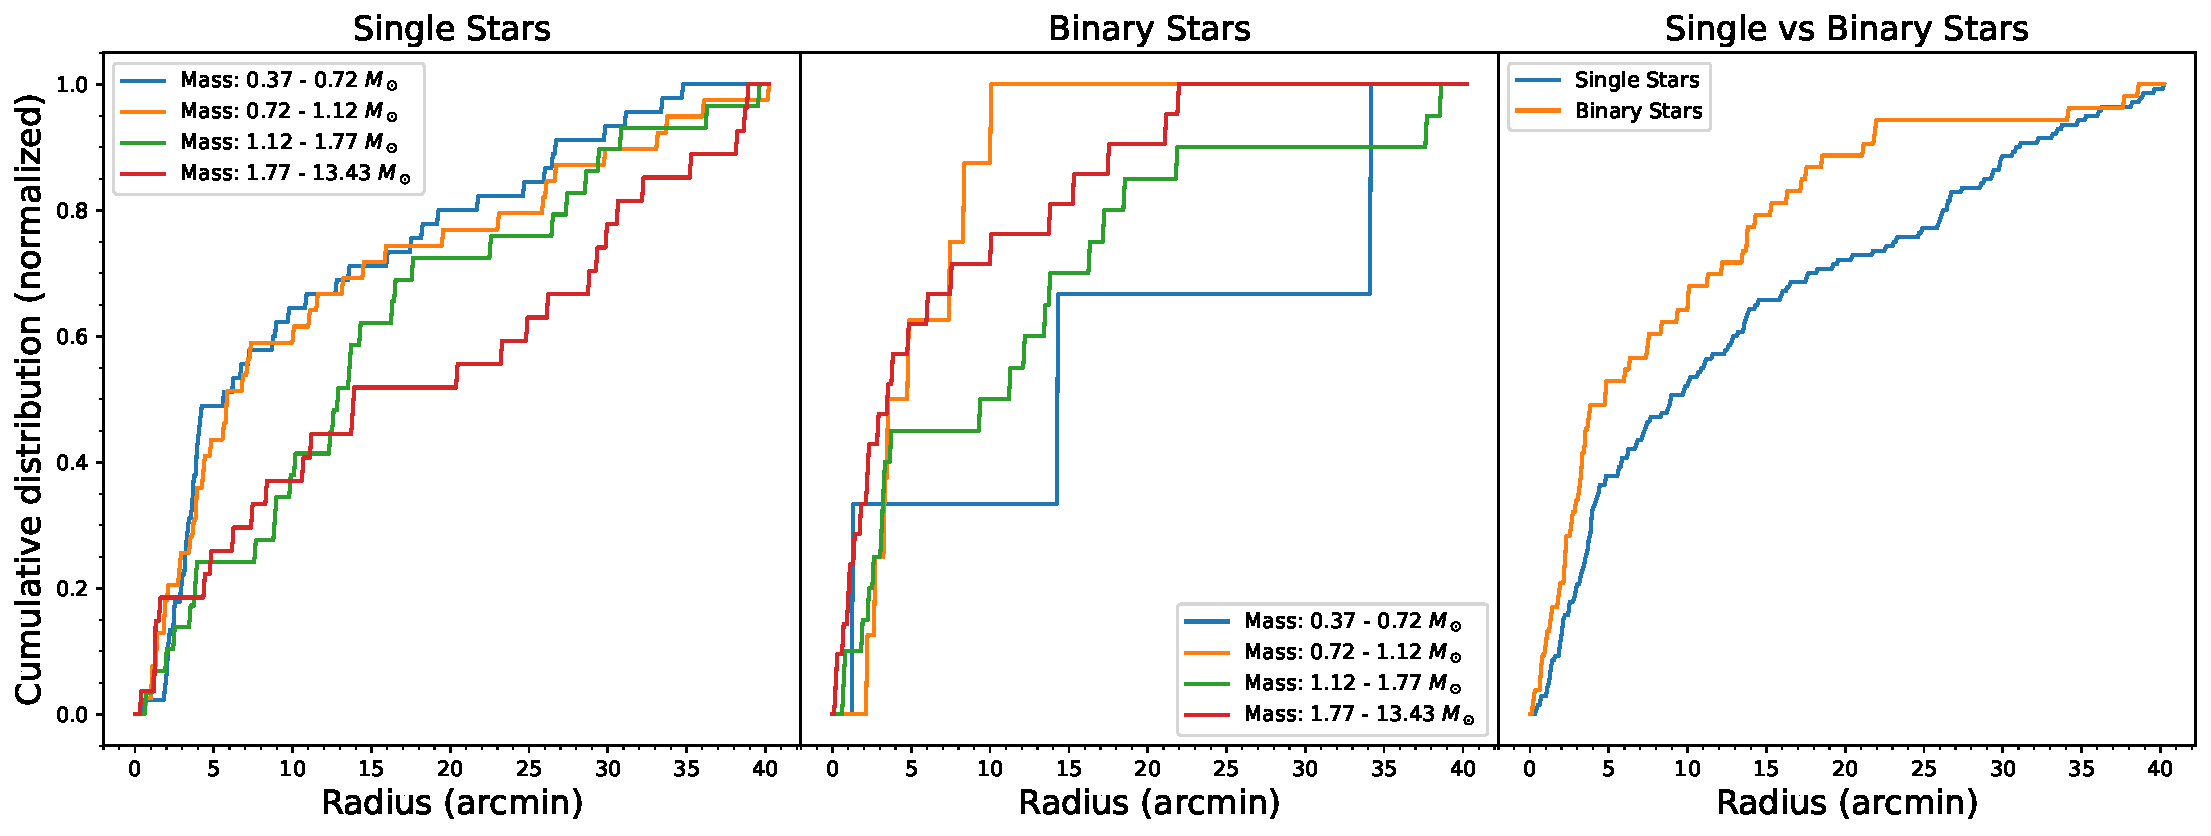
\includegraphics[width=\textwidth]{Figures/cumulative_by_mass_and_type.pdf}
	\caption{\emph{Left panel:} Cumulative distributions of single stars within NGC 6383 are segmented into four mass quartiles ranging from $0.23 - 0.69 M_\odot$ to $1.52 - 13.08 M_\odot$, illustrating the spatial distribution across different mass segments and highlighting the potential influences of mass on stellar distribution within the cluster. \emph{Middle panel:} Similar distributions for binary stars are displayed. \emph{Right panel:} The normalized cumulative distributions compare single versus binary stars, emphasizing differences within the cluster. All plots are based on stars with a membership probability of at least $60$ per cent. Kolmogorov-Smirnov test results are included to quantitatively assess the differences in distributions, underscoring the statistical validity of observed segregation patterns. For a detailed discussion of the Kolmogorov-Smirnov test results, please refer to the main text.}
	\label{fig:mass_seg}
\end{figure*}
\begin{figure}
	\centering
	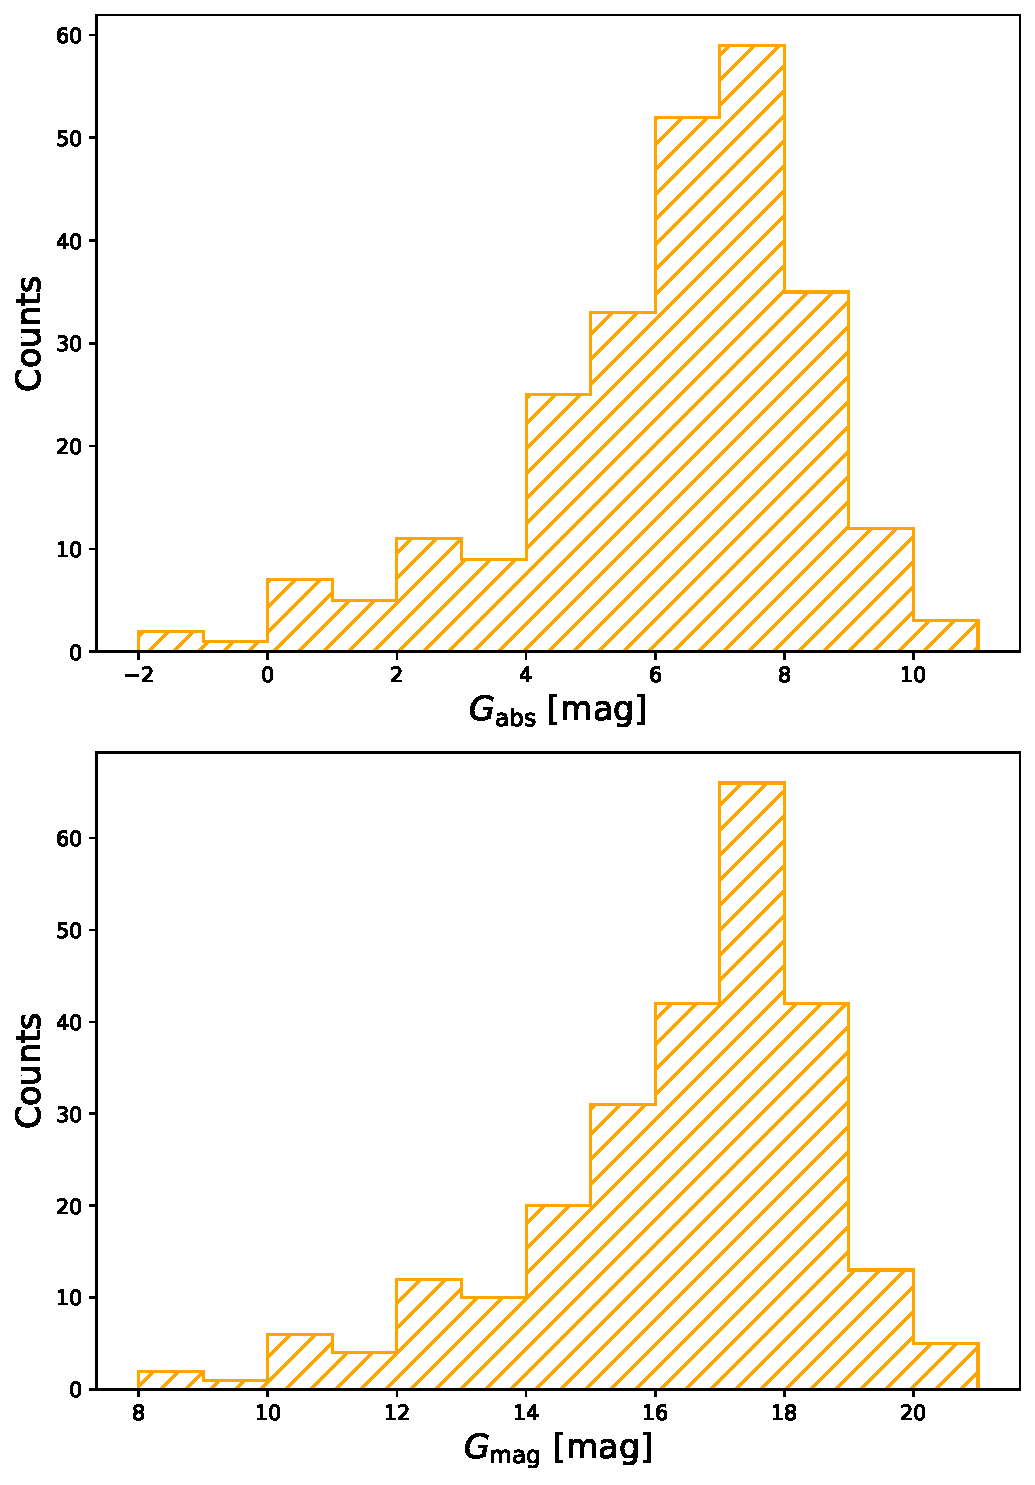
\includegraphics[width=\columnwidth]{Figures/luminosity_function.pdf}
	\caption{\emph{Upper Panel:} Histogram representing the distribution of absolute magnitudes ($ G_{\text{abs}} $) for stars in NGC 6383 that have a membership probability of at least $60$ per cent. \emph{Lower Panel:} Histogram of apparent magnitudes ($ G_{\text{mag}} $) for the same subset of stars, illustrating the observed magnitudes.}
	\label{fig:lf}
\end{figure}
\subsection{Structural Parameters}

The cluster exhibits a tidal radius of $40.712 \pm 14.379\,\mathrm{arcmin}$. The core radius, indicating the densest region, is $1.943 \pm 0.1857\,\mathrm{arcmin}$. The parameters $ k $ and $ b $, representing the King model structural constants, are $4.902 \pm 0.413$ and $0.011 \pm 0.0062$ stars per square arcminute, respectively. These results are visualized in Fig. \ref{fig:king}. The concentration parameter $ C $, defined as $ \log(R_t/R_c) $, is approximately $3.042$, calculated following \citet{1975AJ.....80..427P}. The half-light radius is determined to be $6.023\,\mathrm{arcmin}$.

The cluster's outer limits extend to approximately $40.236\,\mathrm{arcmin}$, as shown in Fig. \ref{fig:center}. We identified $38$ sources between the Hill radius and the tidal radius, with membership probabilities ranging from $0.6$ to $1$, averaging $0.82$. These sources, depicted in Fig.\ref{fig:real_sky}, are likely not gravitationally bound to the cluster due to the extensive area covered by the cone search, implying they share similar proper motion but are not necessarily physically associated with the cluster.

\subsection{Age, Extinction, and Color-Magnitude Diagram}

The Color-Magnitude Diagram (CMD) of NGC 6383 is displayed in Fig. \ref{fig:cmd}, including Pre-Main Sequence (PMS) stars and the median and mean isochrone. The optimal model suggests a logarithmic age of $6.54 \pm 0.155$, a distance modulus of $10.416 \pm 0.748$ corresponding to a distance of $1.211_{0.858}^{1.709}\,\mathrm{kpc}$, and a metallicity $ Z $ of $0.023 \pm 0.008$. An extinction correction of $A_V= 1.221 \pm 0.241$ was applied. The model's modulus distance aligns with our parallax-derived estimates.

The CMD, particularly sources brighter than G magnitude of $12\,\mathrm{mag}$, displays a well-defined main sequence. The presence of PMS stars and lower-mass main sequence stars broadens the lower part of the CMD, complicating the fit of a single isochrone. Figure \ref{fig:cmd_ngc6383_various} presents various isochrones for Gaia and 2MASS data, considering ages between $6.2$ and $7.0$ in logarithmic scale and initial metallicities $ Z $ of $0.023$. The age range of star formation in NGC 6383 appears to span from $6.2$ to $6.8$ in logarithmic scale.

Figure \ref{fig:cmd_ngc6383_various} also includes color-color diagrams $(G_\mathrm{BP} - G_\mathrm{RP})$ showing a clearer segregation of PMS stars, which tend to be at redder colors, as expected. Additionally, Fig. \ref{fig:pms_sagitta_stats} shows the returned Sagitta parameters, which include PMS probability, age, and $A_V$. The posterior distribution of the inferred parameters can be seen as a plot pair in Fig. \ref{fig:plot_pair_trace}.

\subsection{Identification of YSOs}

Our analysis aims to quantify the fraction of Young Stellar Objects (YSOs) within the cluster, noted as $ Y_{\text{frac}} $, which serves as an age indicator. We determined the reddening-free parameter $ Q $ for each star using the formula:
\begin{equation}
	Q = (J - H) - \frac{E(J-H)}{E(H - K)} (H-K)
\end{equation}
where $ E(J-H)/E(H-K) $ is assumed to be $1.55$ \citep{1990ARA&A..28...37M}. Following \citet{2013MNRAS.436.1465B}, a star is considered a YSO if its $ Q $ value is less than $-0.05\,\mathrm{mag}$.

To estimate the lower limit of $ Y_{\text{frac}} $, we assume the presence of at least $ N_{\text{YSO}} - \sqrt{N_{\text{YSO}}} $ young stars, accounting for potential photometric scatter and the typically small numbers of YSOs. The fraction is calculated as
\begin{equation}
	Y_{\text{frac}} = \frac{N_{\text{YSO}} - \sqrt{N_{\text{YSO}}}}{N_{\text{cl}}},
\end{equation}
where $ N_{\text{YSO}} $ is the number of YSOs $ \sqrt{N_{\text{YSO}}} $ represents the uncertainty due to potential photometric scatter, and $ N_{\text{cl}} $ is the total number of cluster members.

We identified $53$ YSOs, with a mean $ Q $ value of $-0.52$, a median of $-0.38$, and a standard deviation of $0.42$ for sources below $-0.05\,\mathrm{mag}$. The resulting $ Y_{\text{frac}} $ is $0.18$, which is higher compared to clusters analyzed in \citet{2013MNRAS.436.1465B}.
\begin{figure*}
	\centering
	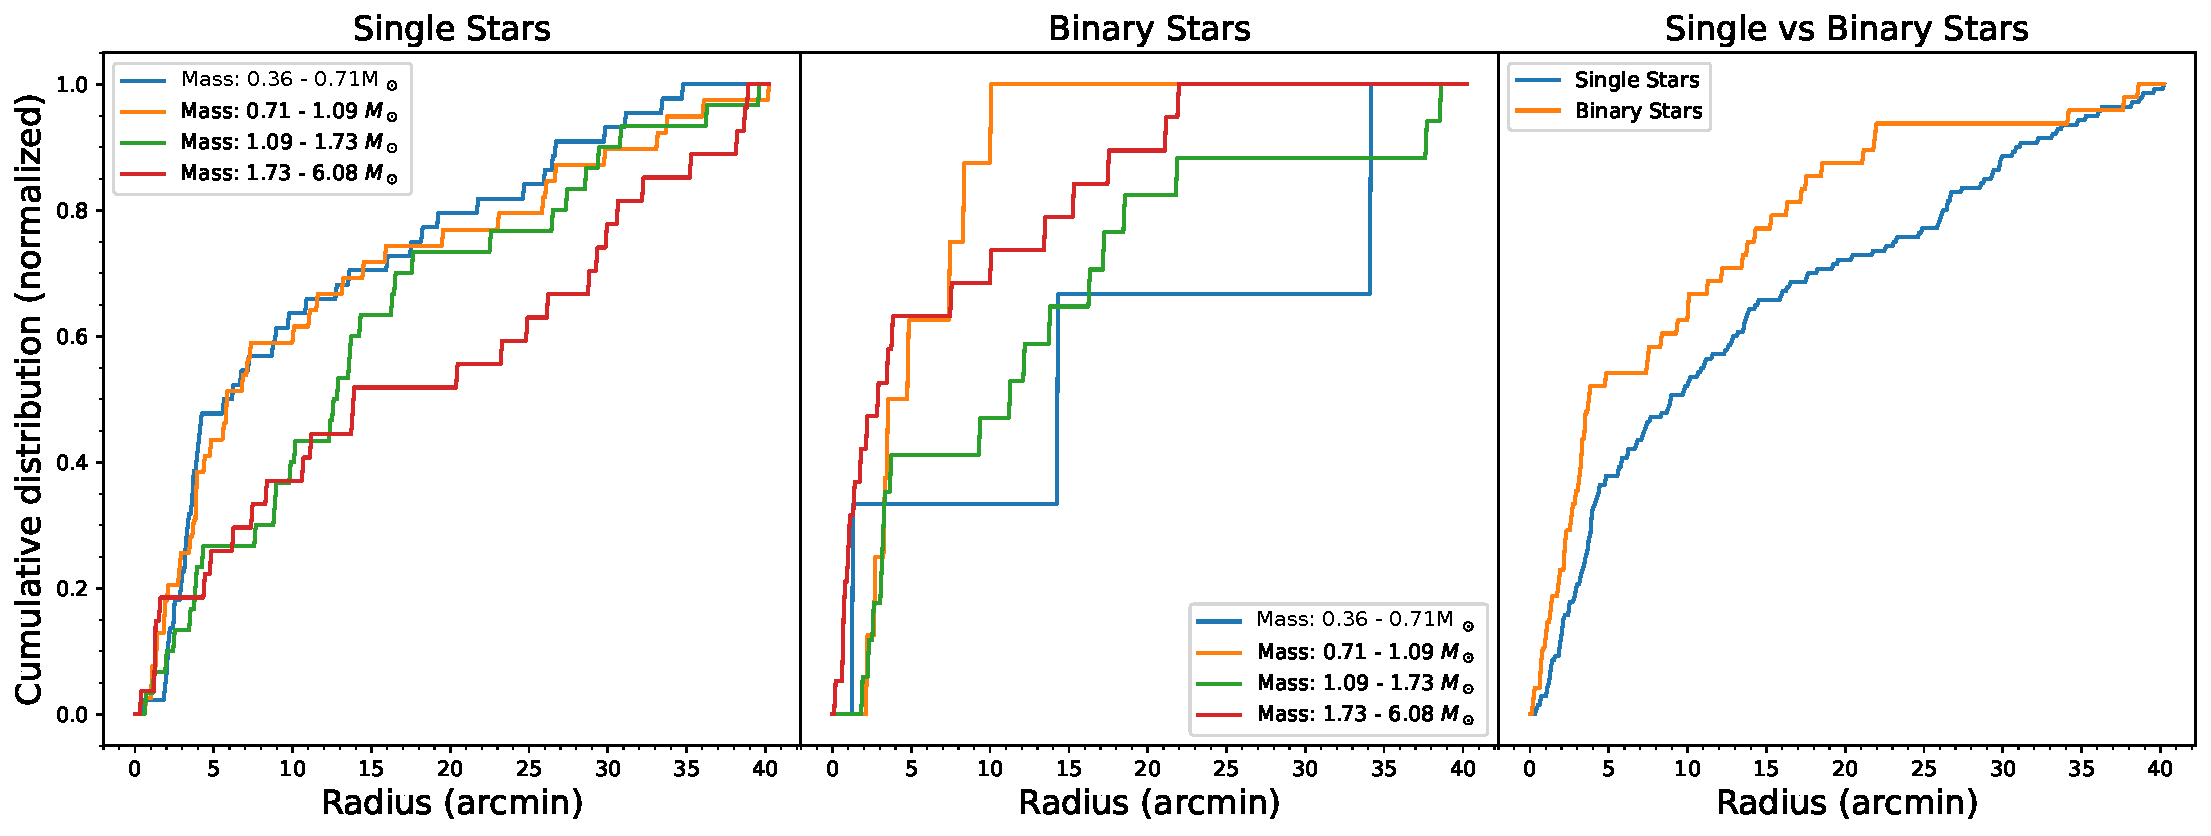
\includegraphics[width=\textwidth]{Figures/cumulative_by_mass_and_type_mseg.pdf}
	\caption{\emph{Left panel:} Same as Fig. \ref{fig:mass_seg}, with cumulative distributions of single stars within NGC 6383. \emph{Middle panel:} Similar distributions for binary stars. \emph{Right panel:} The normalized cumulative distributions compare single versus binary stars. These plots were generated with data filtered for a minimum segment mass cutoff of $2.92 M_\odot$, corresponding to a segregation time of 4 Myr. For a detailed discussion of the K-S test results, please refer to the main text.}
	\label{fig:mass_tseg}
\end{figure*}

\subsection{Luminosity, Mass, and Dynamical State}

The luminosity function (LF) represents the distribution of a cluster's stars across different magnitude bins. For NGC 6383, we converted apparent $G$ magnitudes to absolute magnitudes using the parallax-derived distance. Figure \ref{fig:lf} shows the LF, indicating an increase towards dimmer magnitudes, alongside the luminosity function derived from apparent magnitudes.

The radial cumulative distributions of cluster members at various magnitude levels (Fig. \ref{fig:cumulative_luminosity}) show that fainter stars ($17.93 - 20.66\,\mathrm{mag}$) are less concentrated around the cluster's center. This observation is consistent with Gaia's completeness limit for magnitudes between $18$ and $19$ at distances around $1\,\mathrm{kpc}$ \citep{2020MNRAS.497.4246B,2023AA...677A..37C}. The significance of this distribution was confirmed using a Kolmogorov-Smirnov (K-S) test, yielding p-values from $0.009$ to $0.052$ when compared with other ranges.

AsTeCA calculates the probability of a star being part of a binary system and estimates the masses of the primary and secondary stars. However, these estimates are less reliable in the PMS stage due to the poorly defined CMD, as previously discussed. Figure \ref{fig:cmd_mass_binary} displays these binary probabilities and total mass, indicating that these values should be interpreted with caution, as they may not be entirely accurate. The average mass of the stars is $1.26\,M_\odot$. 

To investigate mass segregation, we constructed radial normalized cumulative mass distributions for single stars, binary stars, and both combined (Fig. \ref{fig:mass_seg}). The K-S test was employed to compare these distributions, indicating a significant difference between binary and single stars, with a p-value of $0.026$ and a K-S test statistic of $0.2079$. This suggests binary mass segregation, where binary stars are more centrally concentrated.  Additionally, the bin mass range between $1.52 - 13.08~M_\odot $ shows a significant difference compared to the other mass ranges, with a p-values ranging from $0.0683$ to $0.0840$ and a K-S test statistic of $\sim 0.2760$, but this mass range is broad and cannot ensure mass segregation within it.

To contextualize these findings, we calculated the half-mass relaxation time ($t_{\mathrm{rh}}$):

\begin{equation}
	t_{\mathrm{rh}} = \frac{0.17N}{\ln(\lambda N)}\sqrt{\frac{r_h^3}{GM}}
\end{equation}

where $N$ is the number of cluster members, $\lambda$ is a constant according to \citet{1994MNRAS.268..257G}, and $r_\mathrm{hm} = 1.65\,\mathrm{pc}$ is the half-mass radius, derived from the radial cumulative mass distribution. The calculated half-mass relaxation time for NGC 6383 is $9.808\,\mathrm{Myr}$.

For estimating the minimum mass segregation time ($t_{\mathrm{seg}}$) for the cluster's most massive star, we follow the approach of \citet{1969ApJ...158L.139S}:

\begin{equation}
t_{\mathrm{seg}} = \frac{\langle m \rangle}{m}t_{rh}
\end{equation}

where $\langle m \rangle$ is the average mass of a star in the cluster, and $m$ is the mass of the most massive star. This results in a segregation time of $1.364\,\mathrm{Myr}$ for the most massive star of $13.08\,M_\odot$, indicating it has had sufficient time to undergo mass segregation.

Finally, we evaluated the potential for primordial mass segregation by comparing the radial distributions of stars with $t_{seg} > 4\,\mathrm{Myr}$ to the cluster's age of approximately $4\,\mathrm{Myr}$. The sample includes stars with masses ranging from $0.22\,M_\odot$ to $3.42\,M_\odot$, and the analysis revealed a similar behavior as the Fig. \ref{fig:mass_seg}, the highest mass bin has a different distribution. In this case, the mass range is not broad, with p-values of $0.0653$ to $0.3364 $ and a K-S test statistic of $0.1976$ to $0.2697$, which indicates primordial mass segregation of the higher mass single sources between the range of $1.39\,M_\odot$ and $3.42\,M_\odot$. In this sample, the average mass is $1.05\,M_\odot$. The distributions of single and binary stars are similar up to approximately $5\,\mathrm{arcmin}$, beyond which single stars show less concentration compared to binary stars.

\subsection{Comparative analysis with cluster members and PMS study}

\subsubsection{Peculiar Stars}

NGC 6383 22 \footnote{Cataloged in Simbad as \textsc{Gaia DR3 4054615634716139264}}, is identified as a $\lambda$ Bootis star. These stars are chemically peculiar A-type stars with abundance anomalies attributed to the accretion of metal-poor material. In a spectroscopic survey of metal-weak and emission-line stars in the Southern Hemisphere, \citet{2020MNRAS.499.2701M} found that $\lambda$ Boo stars, including NGC 6383 22, exhibit excesses at longer wavelengths, suggestive of circumstellar discs. This characteristic aligns with other stars in NGC 6383 and those studied in \citet{2019MNRAS.484.5102K}. Unfortunately, NGC 6383 22, despite matching the position and parallax of the cluster, does not belong to NGC 6383 due to its differing proper motion, indicating it is passing near or through the cluster.
\begin{figure}
	\centering
	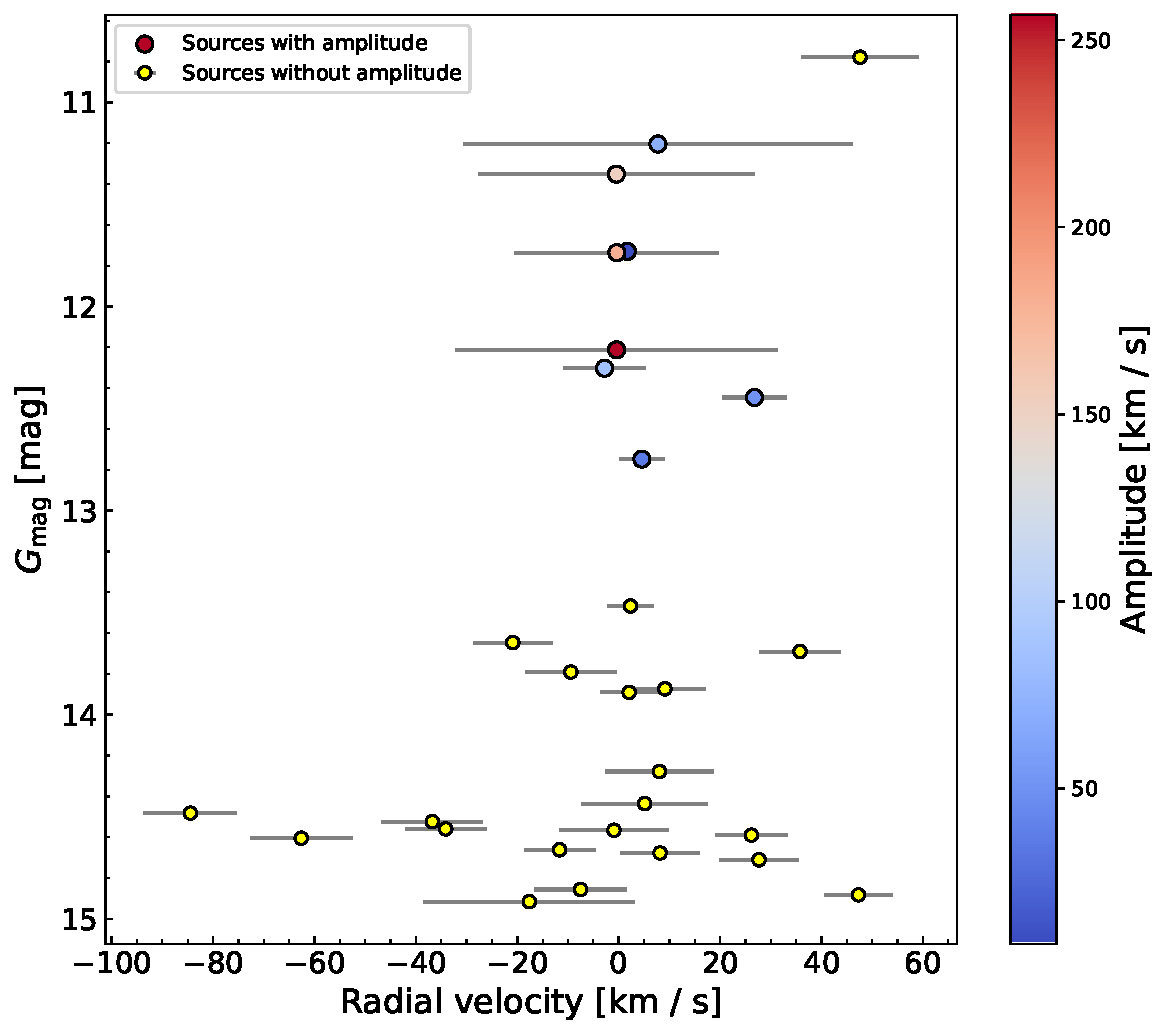
\includegraphics[width=\columnwidth]{Figures/radial_velocity_amplitude.pdf}
	\caption{Radial velocity plotted against G-band magnitude for NGC 6383 sources categorized by the presence of robust radial velocity amplitude data from Gaia. This measure reflects the total amplitude in the radial velocity time series following outlier removal. Yellow circles indicate sources without amplitude measurements, displaying radial velocity uncertainties with error bars. Blue circles represent sources with amplitude data, color-coded by amplitude value according to the scale on the right. This representation allows for detailed analysis of amplitude variations relative to radial velocities and magnitudes in the cluster.}
	\label{fig:radial_velocities}
\end{figure}
\subsubsection{HD 159176}
HD 159176, a double-lined spectroscopic binary composed of O7V type stars, is located in the projected center of NGC 6383 and is responsible for ionizing the surrounding HII region \citep{2016ApJ...832..211P}. The estimated age of HD 159176 is around $2.3-2.8$\,Myr \citep{2010AA...511A..25R}. Previous analyses suggested that HD 159176 might predate the cluster itself and could have initiated star formation in the cluster's core and surrounding areas \citep{1978MNRAS.182..607F}.

In the study by \citet{2018AA...610A..30A}, it was hypothesized that if HD 159176 were a blue straggler, it would imply an older age for NGC 6383, ranging between $6$ and $10$\,Myr. However, our findings indicate that HD 159176 is not a member of NGC 6383. The proper motion of HD 159176 ($\mu_\alpha^* = 2.621 \pm 0.010$ mas yr$^{-1}$, $\mu_\delta = -0.797 \pm 0.009$ mas yr$^{-1}$) differs from the mean proper motion of the cluster. Additionally, the parallax of HD 159176 ($1.153 \pm 0.024$ mas) is outside the $2\sigma$ range of the cluster's parallax distribution.

Despite its central position, these discrepancies in proper motion and parallax confirm that HD 159176 is not gravitationally bound to NGC 6383. Therefore, the hypothesis that HD 159176 is a blue straggler influencing the cluster's age must be reconsidered. Our study supports the notion that NGC 6383 has an age of approximately 4 Myr, independent of HD 159176's characteristics.
\subsubsection{PMS Study Using VPHAS+}

\citet{2019MNRAS.484.5102K} examined 55 classical T-Tauri stars (CTTS) in the star-forming region Sh 2-012 and NGC 6383, utilizing optical photometry and Gaia astrometry. They reported a median age of $2.8 \pm 1.6\,\mathrm{Myr}$ for these stars, with masses ranging from $0.3$ to $1\,M_\odot$. Notably, $94\%$ of CTTS with near-infrared cross-matches conform to the near-infrared T-Tauri locus, and all stars with mid-infrared photometry showed signs of accreting circumstellar discs concentrated around NGC 6383.

Out of the 55 CTTS, only 15 are catalogued as members or potential members in this study, with most having a PMS probability over $0.6$ \footnote{Except for Gaia DR3 4054615467234669440, Gaia DR3 4054617116502154368, Gaia DR3 4054618761456141056, and Gaia DR3 4054826809671572096, which have lower probabilities of $16$, $12$, $55$, and $45$ per cent respectively}. Only one T-Tauri source \footnote{Catalogued as Gaia DR3 4054567805963940352} is likely a binary, with a $0.82$ probability of being a binary star according to our findings.

\subsubsection{Catalogs Comparison}

We compared our membership list with the catalogs from \citet{2020AA...640A...1C}, \citet{2021ApJ...923..129J}, \citet{2022ApJS..262....7H}, \citet{2024arXiv240305143H}, and the members listed in SIMBAD.

From \citet{2020AA...640A...1C}, we identified 148 common sources, found 97 sources not cross-matched in their catalog, and 173 sources unique to our data. \citet{2021ApJ...923..129J} showed 161 sources in common, with 123 sources not present in our data, and 160 not listed in their catalog. The catalog of \citet{2022ApJS..262....7H} includes 90 common sources, 47 not found in our data, and 231 not in their catalog. \citet{2024arXiv240305143H} had 202 common sources, with 120 unique to their catalog, and 119 unique to our results. Using the SIMBAD database, we confirmed 168 common sources, with 163 unique to SIMBAD and 153 unique to our results.

\section{Conclusion}

This study provides a comprehensive analysis of the open cluster NGC 6383, leveraging a combination of Bayesian analysis and machine learning techniques to identify cluster members and determine key parameters. Using the HDBSCAN algorithm, we identified 321 likely cluster members with membership probabilities exceeding 60 percent.

Our findings indicate a mean cluster age of approximately $4~\mathrm{Myr}$, with a distance of $1.207~\mathrm{kpc}$ derived from both parallax and distance modulus methods. We determined the cluster's core and tidal radii to be $1.95~\mathrm{arcmin}$ and $40.53 \mathrm{arcmin}$, respectively, and observed significant mass segregation, particularly among binary stars.

The CMD analysis revealed a well-defined main sequence and a population of PMS stars, highlighting the cluster's recent star formation activity. The Sagitta neural network provided further insights into PMS probabilities, ages, and extinctions of the cluster members.

Comparison with historical data and previous studies shows our results align well with recent estimates, offering updated parameters for NGC 6383. The cluster's structural and dynamic properties, including proper motions, radial velocities, and spatial distribution, were thoroughly characterized, contributing valuable data for future research on young open clusters.

We observed that the binary stars are more centrally concentrated compared to single stars, suggesting both dynamical and primordial mass segregation. The calculated half-mass relaxation time is approximately $9.8~\mathrm{Myr}$, indicating that NGC 6383 is not yet fully relaxed. The observed central concentration of binaries, even for those with segregation times longer than the cluster's age, suggests that these stars may have formed closer to the cluster center or within rapidly evolving clumps that merged early in the cluster's history.

Overall, this study demonstrates the effectiveness of combining advanced computational techniques with traditional astronomical methods to enhance our understanding of stellar clusters. The detailed characterization of NGC 6383 provides a solid foundation for further investigations into its formation history and evolution.

\section*{Acknowledgements}

We gratefully acknowledge support by the ANID BASAL project FB210003 and the SOCHIAS GEMINI project 32230014.

This work has made use of data from the European Space Agency (ESA) mission {\it Gaia} (\url{https://www.cosmos.esa.int/gaia}), processed by the {\it Gaia} Data Processing and Analysis Consortium (DPAC, \url{https://www.cosmos.esa.int/web/gaia/dpac/consortium}). Funding for the DPAC has been provided by national institutions, in particular the institutions participating in the {\it Gaia} Multilateral Agreement. 

This publication makes use of data products from the Two Micron All Sky Survey, which is a joint project of the University of Massachusetts and the Infrared Processing and Analysis Center/California Institute of Technology, funded by the National Aeronautics and Space Administration and the National Science Foundation. This work made use of Astropy:\footnote{http://www.astropy.org} a community-developed core Python package and an ecosystem of tools and resources for astronomy \citep{astropy:2013, astropy:2018, astropy:2022}.

\section*{Data Availability}

\bibliographystyle{mnras}
\bibliography{cites} 

\appendix

\section{Some extra material}
\begin{figure}
	\centering
	
\includegraphics[width=\columnwidth]{Figures/min_cluster_size.pdf}
	\caption{Cluster size variation as a function of minimum cluster size, determined through HDBSCAN clustering on proper motion data of sources. The blue line represents cluster sizes achieved at various minimum cluster sizes. The dashed blue line highlights the optimal minimum cluster size of 43, where the cluster size reaches a peak. The dashed green line indicates the maximum observed cluster size of 701.}
	\label{fig:min_cluster_size}
\end{figure}
\begin{figure}
	
\includegraphics[width=\columnwidth]{Figures/condensed_cluster_tree_NGC6383.pdf}
	\caption{The condensed cluster tree exhibits the hierarchical structure of the cluster system, elucidating the proximity or potential merger of clusters as well as their degree of separation. The dendrogram representation displays the cluster hierarchy, wherein the width (and color) of each branch depicts the number of points in the cluster at that level. Specifically, the plot illustrates the NGC 6383 cluster sources on the left side, while the HDBSCAN-identified field sources are situated on the right side. The color bar corresponds to the number of sources at each level, while the $\lambda$ value corresponds to $\frac{1}{\texttt{distance}}$.}
	\label{fig:condensed_cluster_tree}
\end{figure}
\begin{figure*}
		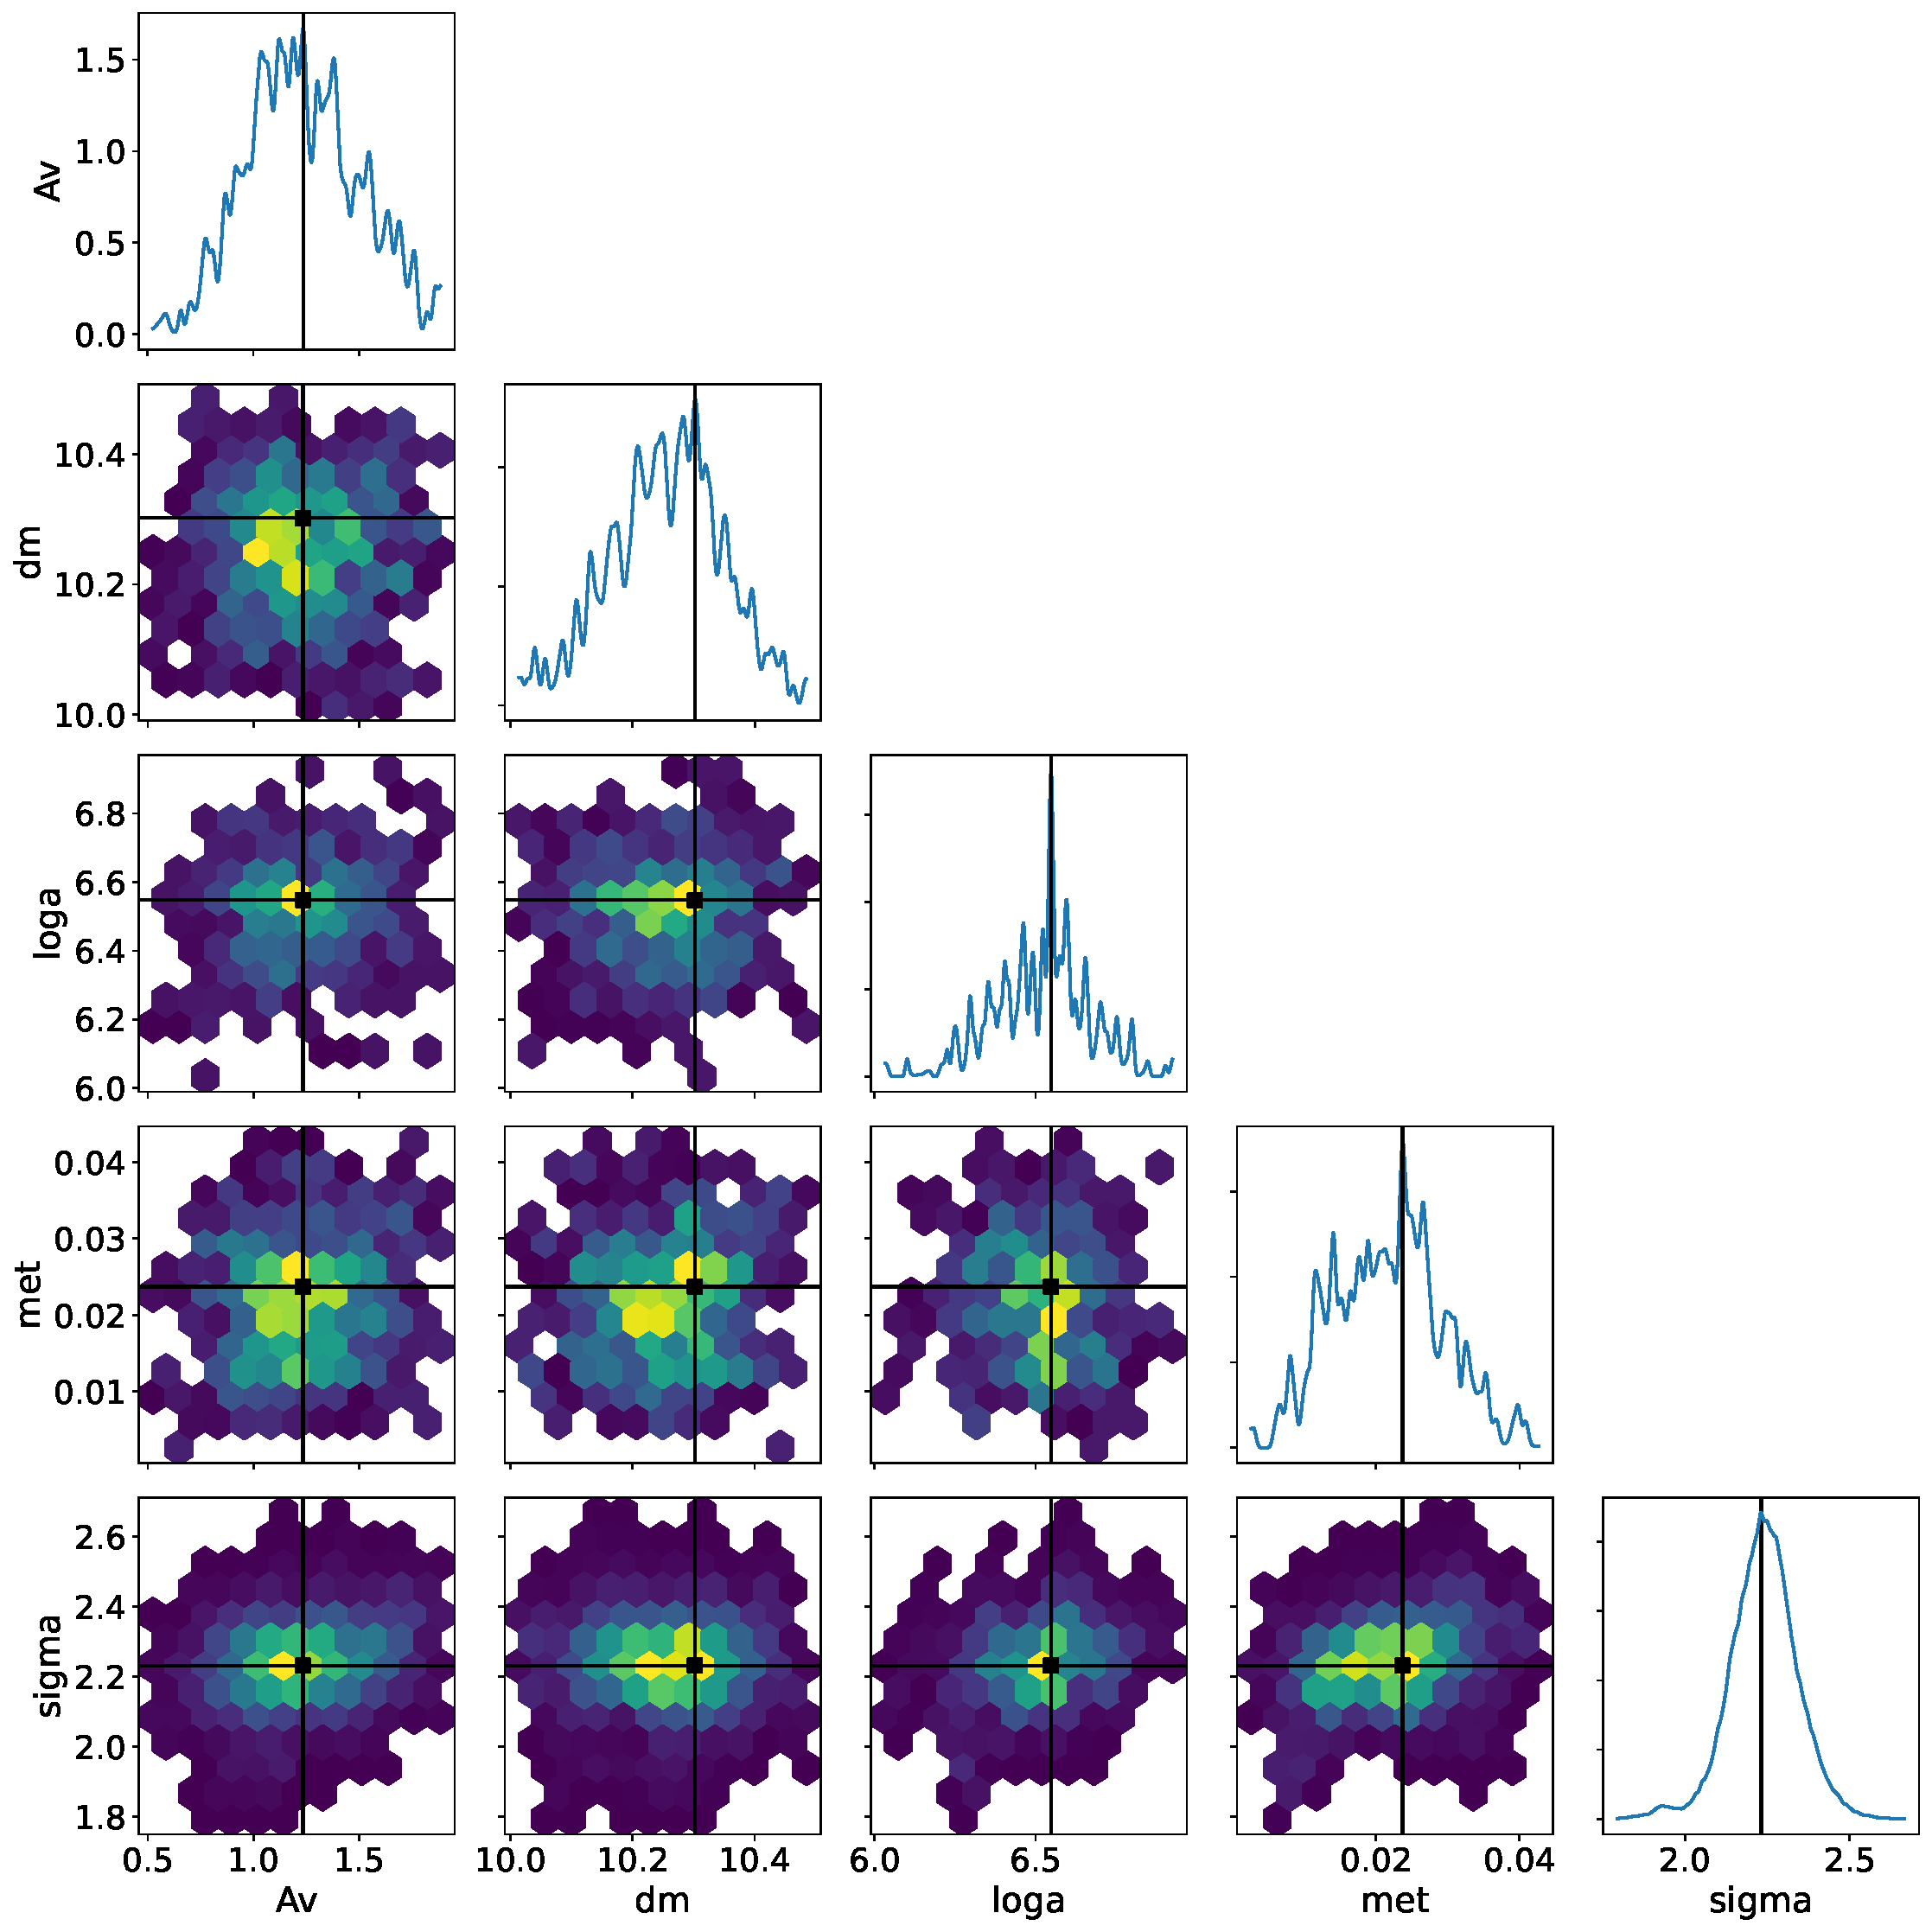
\includegraphics[width=\textwidth]{Figures/plot_pair_trace.pdf}
	\caption{Posterior distributions of the parameters $A_v$ (visual extinction), $dm$ (distance modulus), $loga$ (logarithmic age), and $met$ (metallicity). The diagonals display the marginal distributions for each parameter, showing their individual probability densities. The off-diagonal hexbin plots illustrate the joint distributions, highlighting correlations between parameters. The black lines represent the mode of the distributions.}
	\label{fig:plot_pair_trace}
\end{figure*}
%%%%%%%%%%%%%%%%%%%%%%%%%%%%%%%%%%%%%%%%%%%%%%%%%%

% Don't change these lines
\bsp	% typesetting comment
\label{lastpage}
\end{document}

% End of mnras_template.tex
